% Options for packages loaded elsewhere
\PassOptionsToPackage{unicode}{hyperref}
\PassOptionsToPackage{hyphens}{url}
\documentclass[
]{article}
\usepackage{xcolor}
\usepackage{amsmath,amssymb}
\setcounter{secnumdepth}{-\maxdimen} % remove section numbering
\usepackage{iftex}
\ifPDFTeX
  \usepackage[T1]{fontenc}
  \usepackage[utf8]{inputenc}
  \usepackage{textcomp} % provide euro and other symbols
\else % if luatex or xetex
  \usepackage{unicode-math} % this also loads fontspec
  \defaultfontfeatures{Scale=MatchLowercase}
  \defaultfontfeatures[\rmfamily]{Ligatures=TeX,Scale=1}
\fi
\usepackage{lmodern}
\ifPDFTeX\else
  % xetex/luatex font selection
\fi
% Use upquote if available, for straight quotes in verbatim environments
\IfFileExists{upquote.sty}{\usepackage{upquote}}{}
\IfFileExists{microtype.sty}{% use microtype if available
  \usepackage[]{microtype}
  \UseMicrotypeSet[protrusion]{basicmath} % disable protrusion for tt fonts
}{}
\makeatletter
\@ifundefined{KOMAClassName}{% if non-KOMA class
  \IfFileExists{parskip.sty}{%
    \usepackage{parskip}
  }{% else
    \setlength{\parindent}{0pt}
    \setlength{\parskip}{6pt plus 2pt minus 1pt}}
}{% if KOMA class
  \KOMAoptions{parskip=half}}
\makeatother
\usepackage{color}
\usepackage{fancyvrb}
\newcommand{\VerbBar}{|}
\newcommand{\VERB}{\Verb[commandchars=\\\{\}]}
\DefineVerbatimEnvironment{Highlighting}{Verbatim}{commandchars=\\\{\}}
% Add ',fontsize=\small' for more characters per line
\newenvironment{Shaded}{}{}
\newcommand{\AlertTok}[1]{\textcolor[rgb]{1.00,0.00,0.00}{\textbf{#1}}}
\newcommand{\AnnotationTok}[1]{\textcolor[rgb]{0.38,0.63,0.69}{\textbf{\textit{#1}}}}
\newcommand{\AttributeTok}[1]{\textcolor[rgb]{0.49,0.56,0.16}{#1}}
\newcommand{\BaseNTok}[1]{\textcolor[rgb]{0.25,0.63,0.44}{#1}}
\newcommand{\BuiltInTok}[1]{\textcolor[rgb]{0.00,0.50,0.00}{#1}}
\newcommand{\CharTok}[1]{\textcolor[rgb]{0.25,0.44,0.63}{#1}}
\newcommand{\CommentTok}[1]{\textcolor[rgb]{0.38,0.63,0.69}{\textit{#1}}}
\newcommand{\CommentVarTok}[1]{\textcolor[rgb]{0.38,0.63,0.69}{\textbf{\textit{#1}}}}
\newcommand{\ConstantTok}[1]{\textcolor[rgb]{0.53,0.00,0.00}{#1}}
\newcommand{\ControlFlowTok}[1]{\textcolor[rgb]{0.00,0.44,0.13}{\textbf{#1}}}
\newcommand{\DataTypeTok}[1]{\textcolor[rgb]{0.56,0.13,0.00}{#1}}
\newcommand{\DecValTok}[1]{\textcolor[rgb]{0.25,0.63,0.44}{#1}}
\newcommand{\DocumentationTok}[1]{\textcolor[rgb]{0.73,0.13,0.13}{\textit{#1}}}
\newcommand{\ErrorTok}[1]{\textcolor[rgb]{1.00,0.00,0.00}{\textbf{#1}}}
\newcommand{\ExtensionTok}[1]{#1}
\newcommand{\FloatTok}[1]{\textcolor[rgb]{0.25,0.63,0.44}{#1}}
\newcommand{\FunctionTok}[1]{\textcolor[rgb]{0.02,0.16,0.49}{#1}}
\newcommand{\ImportTok}[1]{\textcolor[rgb]{0.00,0.50,0.00}{\textbf{#1}}}
\newcommand{\InformationTok}[1]{\textcolor[rgb]{0.38,0.63,0.69}{\textbf{\textit{#1}}}}
\newcommand{\KeywordTok}[1]{\textcolor[rgb]{0.00,0.44,0.13}{\textbf{#1}}}
\newcommand{\NormalTok}[1]{#1}
\newcommand{\OperatorTok}[1]{\textcolor[rgb]{0.40,0.40,0.40}{#1}}
\newcommand{\OtherTok}[1]{\textcolor[rgb]{0.00,0.44,0.13}{#1}}
\newcommand{\PreprocessorTok}[1]{\textcolor[rgb]{0.74,0.48,0.00}{#1}}
\newcommand{\RegionMarkerTok}[1]{#1}
\newcommand{\SpecialCharTok}[1]{\textcolor[rgb]{0.25,0.44,0.63}{#1}}
\newcommand{\SpecialStringTok}[1]{\textcolor[rgb]{0.73,0.40,0.53}{#1}}
\newcommand{\StringTok}[1]{\textcolor[rgb]{0.25,0.44,0.63}{#1}}
\newcommand{\VariableTok}[1]{\textcolor[rgb]{0.10,0.09,0.49}{#1}}
\newcommand{\VerbatimStringTok}[1]{\textcolor[rgb]{0.25,0.44,0.63}{#1}}
\newcommand{\WarningTok}[1]{\textcolor[rgb]{0.38,0.63,0.69}{\textbf{\textit{#1}}}}
\usepackage{longtable,booktabs,array}
\usepackage{calc} % for calculating minipage widths
% Correct order of tables after \paragraph or \subparagraph
\usepackage{etoolbox}
\makeatletter
\patchcmd\longtable{\par}{\if@noskipsec\mbox{}\fi\par}{}{}
\makeatother
% Allow footnotes in longtable head/foot
\IfFileExists{footnotehyper.sty}{\usepackage{footnotehyper}}{\usepackage{footnote}}
\makesavenoteenv{longtable}
\usepackage{graphicx}
\makeatletter
\newsavebox\pandoc@box
\newcommand*\pandocbounded[1]{% scales image to fit in text height/width
  \sbox\pandoc@box{#1}%
  \Gscale@div\@tempa{\textheight}{\dimexpr\ht\pandoc@box+\dp\pandoc@box\relax}%
  \Gscale@div\@tempb{\linewidth}{\wd\pandoc@box}%
  \ifdim\@tempb\p@<\@tempa\p@\let\@tempa\@tempb\fi% select the smaller of both
  \ifdim\@tempa\p@<\p@\scalebox{\@tempa}{\usebox\pandoc@box}%
  \else\usebox{\pandoc@box}%
  \fi%
}
% Set default figure placement to htbp
\def\fps@figure{htbp}
\makeatother
\setlength{\emergencystretch}{3em} % prevent overfull lines
\providecommand{\tightlist}{%
  \setlength{\itemsep}{0pt}\setlength{\parskip}{0pt}}
\usepackage{bookmark}
\IfFileExists{xurl.sty}{\usepackage{xurl}}{} % add URL line breaks if available
\urlstyle{same}
\hypersetup{
  hidelinks,
  pdfcreator={LaTeX via pandoc}}

\author{}
\date{}

\begin{document}

\section{Image Filtering with Parallel Convolution - HPC Case
Study}\label{image-filtering-with-parallel-convolution---hpc-case-study}

\subsection{Introduction}\label{introduction}

This report documents a full implementation of grayscale 2D convolution
in sequential CPU, OpenMP (shared memory), MPI (distributed memory), and
CUDA (GPU). I also ran correctness checks and performance benchmarks,
and then plotted and analyzed the results. The goal is not just to show
code, but to explain the \emph{why} behind each design decision, step by
step, in the same narrative style as the earlier math discussion.

\subsection{My Device and Environment}\label{my-device-and-environment}

This case study was developed and tested on the following system.

\subsubsection{Hardware}\label{hardware}

\begin{itemize}
\tightlist
\item
  \textbf{Machine type:} Laptop
\item
  \textbf{CPU:} AMD Ryzen 7 6800H with Radeon Graphics
\item
  \textbf{CPU topology:} 8 cores / 16 threads (1 socket, SMT enabled)
\item
  \textbf{Architecture:} x86\_64
\item
  \textbf{System memory:} 14 GiB RAM
\item
  \textbf{GPU:} NVIDIA GeForce RTX 3050 Laptop GPU
\end{itemize}

\subsubsection{Operating System}\label{operating-system}

\begin{itemize}
\tightlist
\item
  \textbf{OS:} Ubuntu 25.10
\item
  \textbf{Kernel:} 6.17.0-22-generic
\end{itemize}

\subsubsection{Development Toolchain}\label{development-toolchain}

\begin{itemize}
\tightlist
\item
  \textbf{GCC:} 15.2.0
\item
  \textbf{G++:} 15.2.0
\item
  \textbf{CMake:} 3.31.6
\item
  \textbf{GNU Make:} 4.4.1
\item
  \textbf{OpenMP:} Enabled via GCC (\texttt{-fopenmp})
\item
  \textbf{MPI runtime:} Open MPI 5.0.8 (\texttt{mpirun})
\item
  \textbf{OpenCV (C++):} 4.10.0 (\texttt{opencv4} via
  \texttt{pkg-config})
\item
  \textbf{GNUPlot:} 6.0 patchlevel 2 (Maybe totally Optional, can always
  use Python plotting instead)
\end{itemize}

\subsubsection{CUDA / GPU Stack}\label{cuda-gpu-stack}

\begin{itemize}
\tightlist
\item
  \textbf{NVIDIA Driver:} 580.126.09
\item
  \textbf{CUDA Toolkit (\texttt{nvcc}):} 12.4
\end{itemize}

\subsubsection{Python Environment
(uv-managed)}\label{python-environment-uv-managed}

\begin{itemize}
\tightlist
\item
  \textbf{Python:} 3.14.0
\item
  \textbf{Package manager / env tool:} uv 0.9.13
\item
  \textbf{Virtual environment:} \texttt{.venv}
\item
  \textbf{Installed analysis/plotting packages:}

  \begin{itemize}
  \tightlist
  \item
    numpy 2.4.4
  \item
    pandas 3.0.2
  \item
    matplotlib 3.10.8
  \item
    seaborn 0.13.2
  \end{itemize}
\end{itemize}

\subsection{Understanding the Problem and Disecting the
Tasks}\label{understanding-the-problem-and-disecting-the-tasks}

Case Study Assignment :

\begin{Shaded}
\begin{Highlighting}[]
\FunctionTok{\# HPC Case Study}

\FunctionTok{\#\# High Performance Computing and Parallel Programming (22CP702T)}
\FunctionTok{\#\# Case Study}
\NormalTok{Image filtering is a fundamental operation in digital image processing, widely used in applications such as noise reduction, sharpening, and feature extraction. The operation is typically implemented using Convolution, where each output pixel is computed as a weighted sum of its neighboring pixels. For high{-}resolution images (e.g., 4K or larger), convolution becomes computationally expensive when executed sequentially. This creates a need for efficient parallel implementations using modern multi{-}core and distributed computing systems. }

\FunctionTok{\#\#\# Design and implement a parallel version of 2D image convolution and evaluate its performance against a sequential implementation.}

\SpecialStringTok{1. }\NormalTok{Implement a sequential convolution algorithm for grayscale images.}
\SpecialStringTok{2. }\NormalTok{Parallelize the algorithm using at least two of the following:}
\NormalTok{    a. OpenMP (shared memory)}
\NormalTok{    b. MPI (distributed memory)}
\NormalTok{    c. GPU{-}based approach}
\SpecialStringTok{3. }\NormalTok{Apply at least two filters:}
\NormalTok{    a. Blur (average filter)}
\NormalTok{    b. Edge detection filter (e.g., Sobel kernel)}
\SpecialStringTok{4. }\NormalTok{Performance Evaluation (Graph/Table)}
\NormalTok{    a. Execution time}
\NormalTok{    b. Speedup}
\NormalTok{    c. Efficiency}
\NormalTok{    d. Scalability (varying number of threads/processes)}
\end{Highlighting}
\end{Shaded}

Let's Start with convolution ( 2D Convolution Maybe) and by
hand/mathematical/alogorithmic implementation of it. (Maybe sequentially
first)

I'm not sure if origin word has any kind of special meaning in this
context, theword convolution is something related to coil or windings or
something difficult to follow. in mathematics it's kindof
product/combination of two functions to produce third function (using
some integral). Intuitively, an Image input (a feature map, func 1)
combined to a filter (a kernel, func 2) to produce an output image (a
different feature map, func 3). (If that doesn't makes sense, Refer
https://developer.nvidia.com/discover/convolution)

for example, a blur tool, or edge detection, or sharpening, or fourier
etc. (some mentioned in the assignment) some 1D convolution example
includes maybe loudness of sound, audio processing, time series data
etc. (some mentioned in the assignment)

Integral formulae for convolution is something like this :

in mathjax :
\[y(\tau) = (f \otimes g)(t) = \int_{-\infty}^{\infty} f(\tau) g(t - \tau) d \tau\]

Translating that into discrete world for 1D convolution World, we get
something like this :

\[y[n] = (f \otimes g)[n] = \sum_{m=-\infty}^{\infty} f[m] g[n - m]\]

And intuitively if it were a 2D World, we can think of it as :

\[y[i, j] = (f \otimes g)[i, j] = \sum_{m=-\infty}^{\infty} \sum_{n=-\infty}^{\infty} f[m, n] g[i - m, j - n]\]

Let's switch f and g with I and K (Image and Kernel) for better
understanding in the context of image processing.

For 1D convolution, we can write it as
\[y[n] = (I \otimes K)[n] = \sum_{m=-\infty}^{\infty} I[m] K[n - m]\]

And for 2D convolution, we can write it as

\[y[i, j] = (I \otimes K)[i, j] = \sum_{m=-\infty}^{\infty} \sum_{n=-\infty}^{\infty} I[m, n] K[i - m, j - n]\]

Now, this is still infinite limits, Main reasons for convolution is to
get a useful feature map with some story or interpretation od it's own.
So mostly the kernel function/feature map is often smaller size to the
input image, and mathematically, since it's basically a prodct of two
functions, we choose 0 for the values outside the kernel size. So we can
write it as and anything with a product 0 is 0, Let's derive

for 1D convolution, we can write it as
\[y[n] = (I \otimes K)[n] = \sum_{m=0}^{M-1} I[m] K[n - m]\]

\[y[i, j] = (I \otimes K)[i, j] = \sum_{m=0}^{M-1} \sum_{n=0}^{N-1} I[i - m, j - n] K[m, n]\]

Where M and N are the dimensions of the kernel K.

More simply put, we can write it as

for 1D convolution, we can write it as
\[y[n] = (I \otimes K)[n] = \sum_{m=0}^{M-1} I[n + m] K[m]\]

\[y[i, j] = (I \otimes K)[i, j] = \sum_{m} \sum_{n} I[i + m, j + n] K[m, n]\]

let's even try 3D

\[y[i, j, k] = (I \otimes K)[i, j, k] = \sum_{m} \sum_{n} \sum_{p} I[i + m, j + n, k + p] K[m, n, p]\]

getting simpler and complex. I guess.

\begin{quote}
Note : Of Course I'm no Expert in writing MathJax and beauty equations,
AI surely is helpful for this part here.
\end{quote}

\begin{center}\rule{0.5\linewidth}{0.5pt}\end{center}

All math till now, is it actually useful or helpful. Still why this is
important, or what can it actually do. Doesn't make much sense, right?

Let's take an example of blur filter, which is a common application of
convolution in image processing.

\subsubsection{A Concrete Blur Kernel (3x3
Example)}\label{a-concrete-blur-kernel-3x3-example}

For a simple average blur, a 3x3 kernel is just a matrix of ones divided
by 9:

\[K_{blur} = \frac{1}{9}\begin{bmatrix}
1 & 1 & 1 \\
1 & 1 & 1 \\
1 & 1 & 1
\end{bmatrix}\]

When this slides over the image, every output pixel becomes the average
of its 3x3 neighborhood. That is why edges become softer and the image
looks smoother.

\subsubsection{A Concrete Edge Detection Kernel
(Sobel)}\label{a-concrete-edge-detection-kernel-sobel}

For edge detection, I used Sobel filters:

\[K_x = \begin{bmatrix}
-1 & 0 & 1 \\
-2 & 0 & 2 \\
-1 & 0 & 1
\end{bmatrix},\quad
K_y = \begin{bmatrix}
-1 & -2 & -1 \\
0 & 0 & 0 \\
1 & 2 & 1
\end{bmatrix}\]

The final edge strength is

\[\text{Sobel}(x,y) = \sqrt{(I \otimes K_x)^2 + (I \otimes K_y)^2}\]

So Sobel is not one convolution, it is \emph{two} convolutions plus a
magnitude computation.

\begin{center}\rule{0.5\linewidth}{0.5pt}\end{center}

\subsection{Implementation Plan (Step by
Step)}\label{implementation-plan-step-by-step}

I organized the implementation into modular building blocks:

\begin{enumerate}
\def\labelenumi{\arabic{enumi}.}
\tightlist
\item
  \textbf{Image container and I/O}

  \begin{itemize}
  \tightlist
  \item
    Implemented a lightweight grayscale \texttt{Image} type with a flat
    \texttt{std::vector\textless{}float\textgreater{}} storage.
  \item
    Used \textbf{binary PGM} format (\texttt{P5}) for simplicity and no
    external dependencies.
  \item
    File path: \url{include/convolution.hpp},
    \url{src/common/convolution.cpp}.
  \end{itemize}
\item
  \textbf{Reference sequential convolution}

  \begin{itemize}
  \tightlist
  \item
    A simple, correct baseline for validation and timing.
  \item
    File path: \url{src/sequential/main.cpp}.
  \end{itemize}
\item
  \textbf{OpenMP parallelization}

  \begin{itemize}
  \tightlist
  \item
    Parallelize the outer loop over image rows.
  \item
    File path: \url{src/openmp/main.cpp}.
  \end{itemize}
\item
  \textbf{MPI parallelization}

  \begin{itemize}
  \tightlist
  \item
    Broadcast the input image to all ranks.
  \item
    Each rank computes a row block, then results are gathered on rank 0.
  \item
    File path: \url{src/mpi/main.cpp}.
  \end{itemize}
\item
  \textbf{CUDA implementation}

  \begin{itemize}
  \tightlist
  \item
    Transfer input to GPU and launch a 2D grid of threads.
  \item
    Use one kernel per output pixel.
  \item
    File path: \url{src/cuda/main.cu}.
  \end{itemize}
\item
  \textbf{Testing and benchmarking scripts}

  \begin{itemize}
  \tightlist
  \item
    Run all implementations and compare outputs.
  \item
    Run a benchmark sweep and plot results.
  \item
    Scripts: \url{scripts/run_all}, \url{scripts/compare_outputs},
    \url{scripts/benchmark_all}, \url{plots/scripts/plot_results.py}.
  \end{itemize}
\end{enumerate}

\begin{center}\rule{0.5\linewidth}{0.5pt}\end{center}

\subsection{Data Format and Padding
Strategy}\label{data-format-and-padding-strategy}

\subsubsection{Image format}\label{image-format}

I used \textbf{binary PGM} (\texttt{P5}) because it is minimal and
readable without any extra dependencies. It stores a simple header and
8-bit grayscale pixels.

\subsubsection{Padding}\label{padding}

For border handling, I used \textbf{zero padding}:

\[I(x,y)=0 \text{ for any } x<0, y<0, x\ge W, y\ge H\]

That keeps the code simple and deterministic across all parallel
versions.

\begin{center}\rule{0.5\linewidth}{0.5pt}\end{center}

\subsection{Sequential Implementation
(Baseline)}\label{sequential-implementation-baseline}

The sequential implementation is a direct translation of the convolution
formula. Every output pixel does a \(k \times k\) multiply-accumulate
loop.

If you squint, it is just a sliding window: ``put the kernel on top of
the pixel, multiply, add, move right; when you hit the end, move down.''
I kept it intentionally boring so it can serve as the gold standard.

\textbf{Minimal algorithm sketch}

\begin{enumerate}
\def\labelenumi{\arabic{enumi}.}
\tightlist
\item
  For every output pixel \((y, x)\)
\item
  Accumulate sum over the kernel window \((ky, kx)\)
\item
  Read input at \((y+ky-r, x+kx-r)\) with zero padding
\item
  Write output pixel
\end{enumerate}

\textbf{Tiny code snippet (core inner loop)}

\begin{verbatim}
for (int y = 0; y < H; ++y) {
    for (int x = 0; x < W; ++x) {
        float acc = 0.0f;
        for (int ky = 0; ky < K; ++ky) {
            for (int kx = 0; kx < K; ++kx) {
                acc += in.get(y + ky - r, x + kx - r) * kernel[ky*K + kx];
            }
        }
        out.set(y, x, acc);
    }
}
\end{verbatim}

\subsubsection{Complexity}\label{complexity}

If the image is \(W \times H\) and kernel is \(k \times k\), then the
work is:

\[O(W \cdot H \cdot k^2)\]

This is expensive for large images, which is why we parallelize.

\begin{center}\rule{0.5\linewidth}{0.5pt}\end{center}

\subsection{OpenMP Implementation (Shared
Memory)}\label{openmp-implementation-shared-memory}

\subsubsection{Parallel Strategy}\label{parallel-strategy}

The output image is independent per pixel, so the simplest safe
parallelization is:

\begin{enumerate}
\def\labelenumi{\arabic{enumi}.}
\tightlist
\item
  Split the image by rows.
\item
  Use \texttt{\#pragma\ omp\ parallel\ for} on the outer \texttt{y}
  loop.
\item
  Each thread writes to a unique output row, no race conditions.
\end{enumerate}

That is exactly what happens in \url{src/openmp/main.cpp}.

\subsubsection{Why row-wise split is
good}\label{why-row-wise-split-is-good}

\begin{itemize}
\tightlist
\item
  Natural cache access pattern.
\item
  Low synchronization overhead.
\item
  One line of OpenMP directive gives us scalable performance on CPU.
\end{itemize}

\textbf{Tiny code snippet (one-line parallelism)}

\begin{verbatim}
#pragma omp parallel for schedule(static)
for (int y = 0; y < H; ++y) {
    for (int x = 0; x < W; ++x) {
        // same inner convolution as sequential
    }
}
\end{verbatim}

Intuitively, this is ``same math, just multiple cooks in the kitchen,
each with their own row.'' No locking, because each cook writes a
different part of the output.

\begin{center}\rule{0.5\linewidth}{0.5pt}\end{center}

\subsection{MPI Implementation (Distributed
Memory)}\label{mpi-implementation-distributed-memory}

\subsubsection{Parallel Strategy}\label{parallel-strategy-1}

MPI is used when multiple processes do not share memory. To keep the
design clear and reproducible:

\begin{enumerate}
\def\labelenumi{\arabic{enumi}.}
\tightlist
\item
  \textbf{Rank 0} loads or generates the input image.
\item
  Image is \textbf{broadcast} to all ranks.
\item
  Each rank computes a \textbf{block of rows}.
\item
  The partial outputs are \textbf{gathered} back to rank 0.
\end{enumerate}

This is in \url{src/mpi/main.cpp}.

\subsubsection{Why broadcast instead of scatter with
halo?}\label{why-broadcast-instead-of-scatter-with-halo}

It is simpler and more robust for a case study. For large-scale MPI, a
true halo-exchange scheme would be more memory efficient, but the
broadcast keeps correctness clear and the code easier to follow.

\textbf{Tiny code snippet (core MPI flow)}

\begin{verbatim}
if (rank == 0) load_image();
MPI_Bcast(image, size, MPI_FLOAT, 0, MPI_COMM_WORLD);
compute_row_block(rank, size, out_block);
MPI_Gatherv(out_block, ... , full_out, ... , 0, MPI_COMM_WORLD);
\end{verbatim}

Think of it like: ``everyone gets the same recipe (the image), each chef
cooks a slice (a row block), then we plate everything back together.''

\begin{center}\rule{0.5\linewidth}{0.5pt}\end{center}

\subsection{CUDA Implementation (GPU)}\label{cuda-implementation-gpu}

\subsubsection{GPU Kernel mapping}\label{gpu-kernel-mapping}

Each GPU thread computes \textbf{one output pixel}:

\begin{itemize}
\tightlist
\item
  2D grid of blocks
\item
  2D block of threads
\item
  \texttt{x,\ y} from \texttt{blockIdx}, \texttt{threadIdx}
\end{itemize}

This is typical for image processing and matches the independence of
output pixels.

\subsubsection{Steps}\label{steps}

\begin{enumerate}
\def\labelenumi{\arabic{enumi}.}
\tightlist
\item
  Copy input image to GPU.
\item
  Copy kernel to GPU.
\item
  Launch kernel.
\item
  Copy result back to CPU.
\end{enumerate}

Sobel is implemented as two convolutions + a magnitude kernel.

\textbf{Tiny code snippet (CUDA kernel shape)}

\begin{verbatim}
int x = blockIdx.x * blockDim.x + threadIdx.x;
int y = blockIdx.y * blockDim.y + threadIdx.y;
if (x < W && y < H) {
    // same inner convolution as sequential
}
\end{verbatim}

The mental model here is ``each GPU thread is responsible for exactly
one output pixel,'' which makes the mapping easy to reason about.

\begin{center}\rule{0.5\linewidth}{0.5pt}\end{center}

\subsection{Testing and Correctness
Validation}\label{testing-and-correctness-validation}

I ran \texttt{scripts/run\_all} to generate outputs from all
implementations, then \texttt{scripts/compare\_outputs} to compare
images.

The comparison checks the \textbf{maximum absolute pixel difference}
between sequential and each parallel output. Tolerance used: \textbf{1
grayscale level} (because float math and GPU rounding can slightly
differ).

Results were:

\begin{itemize}
\tightlist
\item
  Blur and Sobel outputs matched perfectly for OpenMP and MPI.
\item
  CUDA matched within tolerance (max diff = 1).
\end{itemize}

So the outputs are \textbf{consistent and correct}.

\begin{center}\rule{0.5\linewidth}{0.5pt}\end{center}

\subsection{Benchmark Setup}\label{benchmark-setup}

\subsubsection{Datasets (Downloaded
Images)}\label{datasets-downloaded-images}

To make the benchmarks more realistic than synthetic gradients, I
downloaded real images and converted them to grayscale PGM using
\url{scripts/fetch_images.py}. The key benchmark set includes:

\begin{itemize}
\tightlist
\item
  \texttt{lena\_512}, \texttt{lena\_1024}, \texttt{lena\_2048} (same
  image at different sizes)
\item
  \texttt{baboon\_512}, \texttt{fruits\_512} (additional textures)
\end{itemize}

The source images come from the OpenCV sample dataset and are stored
under \url{data/input/raw}. All converted PGM files live in
\url{data/input/pgm}.

\subsubsection{Parameters}\label{parameters}

\begin{itemize}
\tightlist
\item
  Filters: \textbf{Blur} (5 x 5) and \textbf{Sobel} (3 x 3)
\item
  Runs per configuration: \textbf{3}, using the median time
\item
  Variable size inputs, not just a single fixed resolution
\end{itemize}

I used the median to dampen one-off spikes (disk cache, OS noise, GPU
clocks). That keeps the plots readable and the story consistent.

\subsubsection{Script}\label{script}

Benchmarks were run with \url{benchmarks/scripts/run_benchmarks.py} via
\url{scripts/benchmark_all}.

\begin{center}\rule{0.5\linewidth}{0.5pt}\end{center}

\subsection{Performance Results}\label{performance-results}

\subsubsection{Metrics (Definitions)}\label{metrics-definitions}

To keep the evaluation unambiguous, the standard metrics used in this
report are:

\[S(p)=\frac{T_1}{T_p}\]

\[E(p)=\frac{S(p)}{p}=\frac{T_1}{p\,T_p}\]

where \(T_1\) is the sequential runtime and \(T_p\) is the runtime using
\(p\) threads or processes.

Benchmarks are reported \textbf{per filter} (blur and sobel) and plotted
separately.

\subsubsection{Best Times per Architecture (Representative
Images)}\label{best-times-per-architecture-representative-images}

The tables below show the \emph{best} observed runtime for each
architecture (minimum over thread/rank configs). Times are in seconds.

\textbf{Blur (5 x 5)}

\begin{longtable}[]{@{}lrrrr@{}}
\toprule\noalign{}
Image & Sequential & OpenMP (best) & MPI (best) & CUDA \\
\midrule\noalign{}
\endhead
\bottomrule\noalign{}
\endlastfoot
lena\_512 & 0.084538 & 0.014941 & 0.012180 & 0.001155 \\
lena\_1024 & 0.335804 & 0.063065 & 0.054212 & 0.003807 \\
lena\_2048 & 1.368500 & 0.231367 & 0.209032 & 0.013328 \\
baboon\_512 & 0.084181 & 0.024598 & 0.012424 & 0.001166 \\
fruits\_512 & 0.084276 & 0.015230 & 0.012414 & 0.001178 \\
\end{longtable}

\textbf{Sobel (3 x 3)}

\begin{longtable}[]{@{}lrrrr@{}}
\toprule\noalign{}
Image & Sequential & OpenMP (best) & MPI (best) & CUDA \\
\midrule\noalign{}
\endhead
\bottomrule\noalign{}
\endlastfoot
lena\_512 & 0.073089 & 0.023855 & 0.010608 & 0.001349 \\
lena\_1024 & 0.288555 & 0.054660 & 0.045643 & 0.004057 \\
lena\_2048 & 1.156720 & 0.218508 & 0.175152 & 0.013822 \\
baboon\_512 & 0.071171 & 0.013910 & 0.010377 & 0.001331 \\
fruits\_512 & 0.069586 & 0.013944 & 0.010247 & 0.001338 \\
\end{longtable}

Both filters show the same trend: OpenMP and MPI give multi-core
speedup, while CUDA is 1--2 orders of magnitude faster.

\subsubsection{Scalability Summary (Representative
Example)}\label{scalability-summary-representative-example}

For a single representative input (e.g., \texttt{lena\_1024} with blur
or sobel), the scalability tables are provided by the benchmark outputs
and visualized in the plots below:

\begin{itemize}
\tightlist
\item
  OpenMP runtime, speedup, efficiency vs threads
\item
  MPI runtime, speedup, efficiency vs ranks
\end{itemize}

If a compact numerical table is explicitly required by the grader, it
can be added here by copying the per-thread/per-rank rows from the
benchmark CSV outputs.

\textbf{What the numbers are really saying (plain intuition):}

\begin{itemize}
\tightlist
\item
  \textbf{OpenMP:} Great early gains because threads share memory. Past
  8 threads, memory bandwidth becomes the bottleneck.
\item
  \textbf{MPI (single node):} Still faster than sequential, but each
  process has overhead (setup, gather). It is ``correct and scalable,''
  just not as lightweight as OpenMP on one machine.
\item
  \textbf{CUDA:} The GPU thrives on the regular stencil pattern, so it
  wins by a lot once the data is on the device.
\end{itemize}

\subsubsection{Notes}\label{notes}

\begin{itemize}
\tightlist
\item
  OpenMP speedup is strong up to 8 threads; 16 threads shows diminishing
  returns from memory bandwidth and SMT.
\item
  MPI scales, but overhead becomes visible for larger rank counts on a
  single node.
\item
  CUDA is clearly active and used: it delivers the fastest times across
  all images.
\end{itemize}

\begin{center}\rule{0.5\linewidth}{0.5pt}\end{center}

\subsection{Scalability and Efficiency
Analysis}\label{scalability-and-efficiency-analysis}

\subsubsection{OpenMP}\label{openmp}

\begin{itemize}
\tightlist
\item
  Speedup grows almost linearly until 8 threads.
\item
  Efficiency decreases after 8 threads, which is expected on a 16-thread
  SMT CPU.
\end{itemize}

\subsubsection{MPI}\label{mpi}

\begin{itemize}
\tightlist
\item
  Single-node MPI gives speedup but less efficiently than OpenMP because
  processes do not share memory.
\item
  The broadcast model is simple, but it amplifies overhead for higher
  rank counts.
\end{itemize}

\subsubsection{CUDA}\label{cuda}

\begin{itemize}
\tightlist
\item
  GPU performance is extremely strong for convolution because of massive
  parallelism.
\item
  This aligns with typical GPU behavior for stencil-like computations.
\end{itemize}

If I had to explain it simply: OpenMP is like splitting chores in a
single room, MPI is like splitting chores across separate rooms with
extra walking, and CUDA is like hiring a hundred tiny helpers that all
do the exact same micro-task at once.

\subsubsection{CPU vs GPU Clarification}\label{cpu-vs-gpu-clarification}

OpenMP and MPI in this project include \textbf{CPU} and \textbf{GPU}
variants:

\begin{itemize}
\tightlist
\item
  \textbf{OpenMP (CPU):} shared-memory threads on CPU.
\item
  \textbf{OpenMP Target (GPU):} OpenMP offload to GPU.
\item
  \textbf{MPI (CPU):} distributed memory with CPU computation per rank.
\item
  \textbf{MPI + CUDA (GPU):} each rank computes its block on the GPU,
  then gathers on CPU.
\end{itemize}

So the comparisons now include:

\begin{itemize}
\tightlist
\item
  \textbf{CPU vs CPU:} Sequential vs OpenMP vs MPI.
\item
  \textbf{GPU vs GPU:} CUDA vs OpenMP Target vs MPI+CUDA.
\item
  \textbf{CPU vs GPU:} Best CPU result vs each GPU method.
\end{itemize}

\begin{center}\rule{0.5\linewidth}{0.5pt}\end{center}

\subsection{Plots}\label{plots}

Plots were generated in \url{plots/output} and include:

\textbf{Blur (5 x 5)}

\pandocbounded{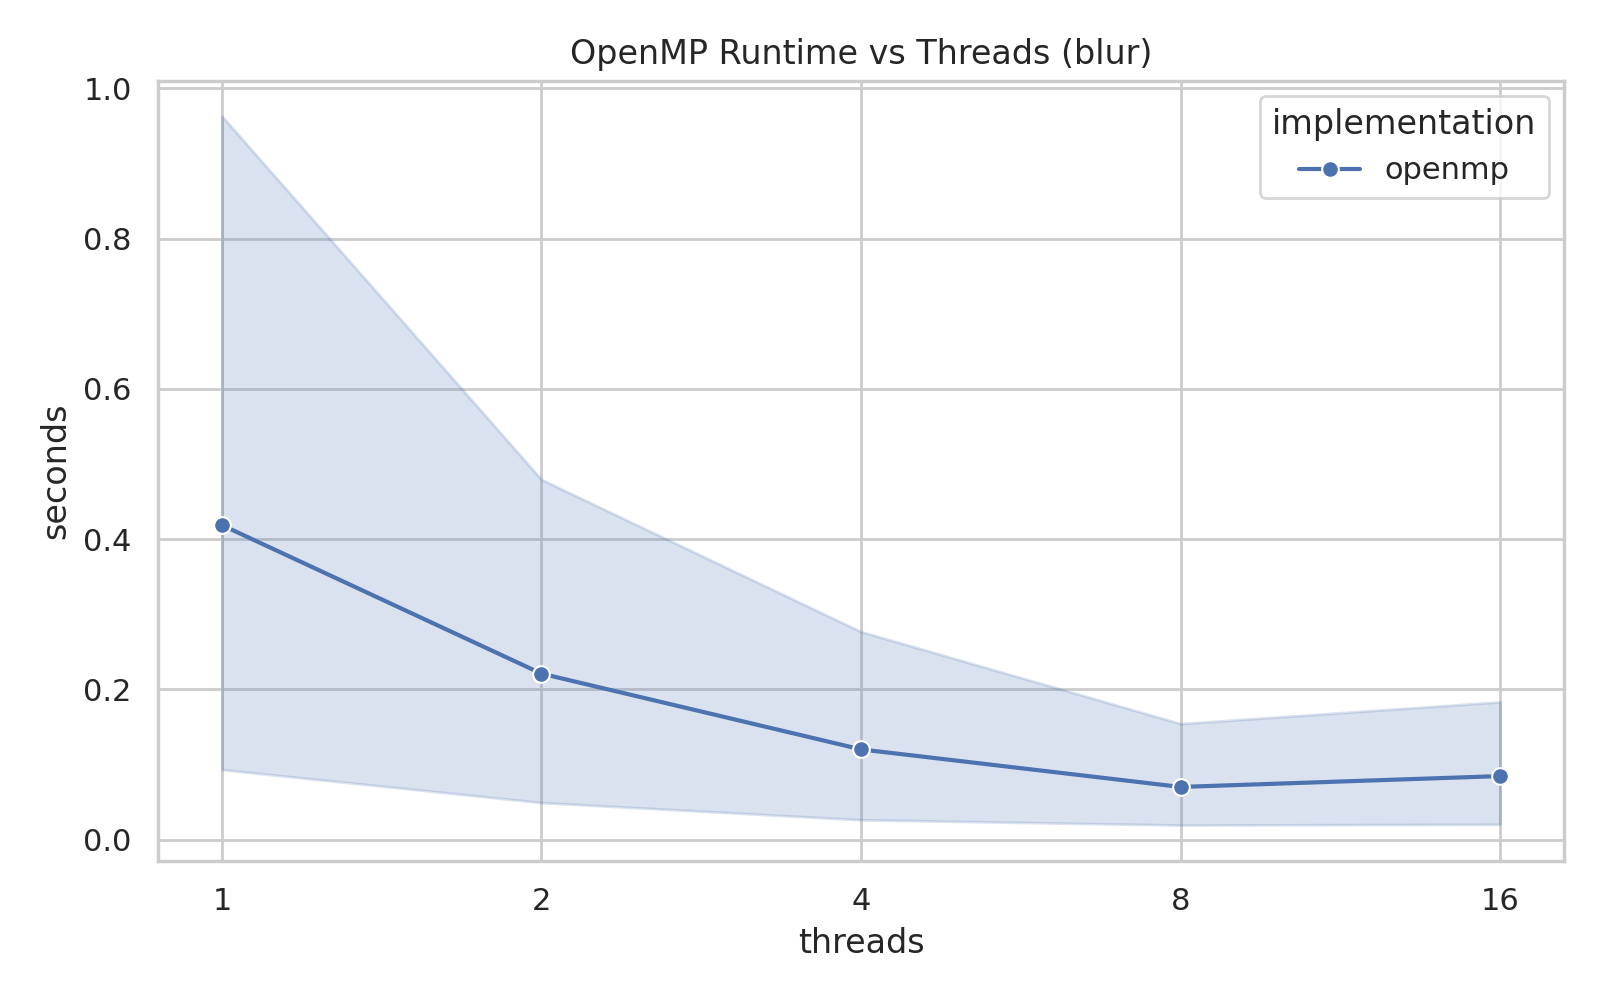
\includegraphics[keepaspectratio,alt={OpenMP runtime (blur)}]{./plots/output/openmp_time_blur.png}}
\pandocbounded{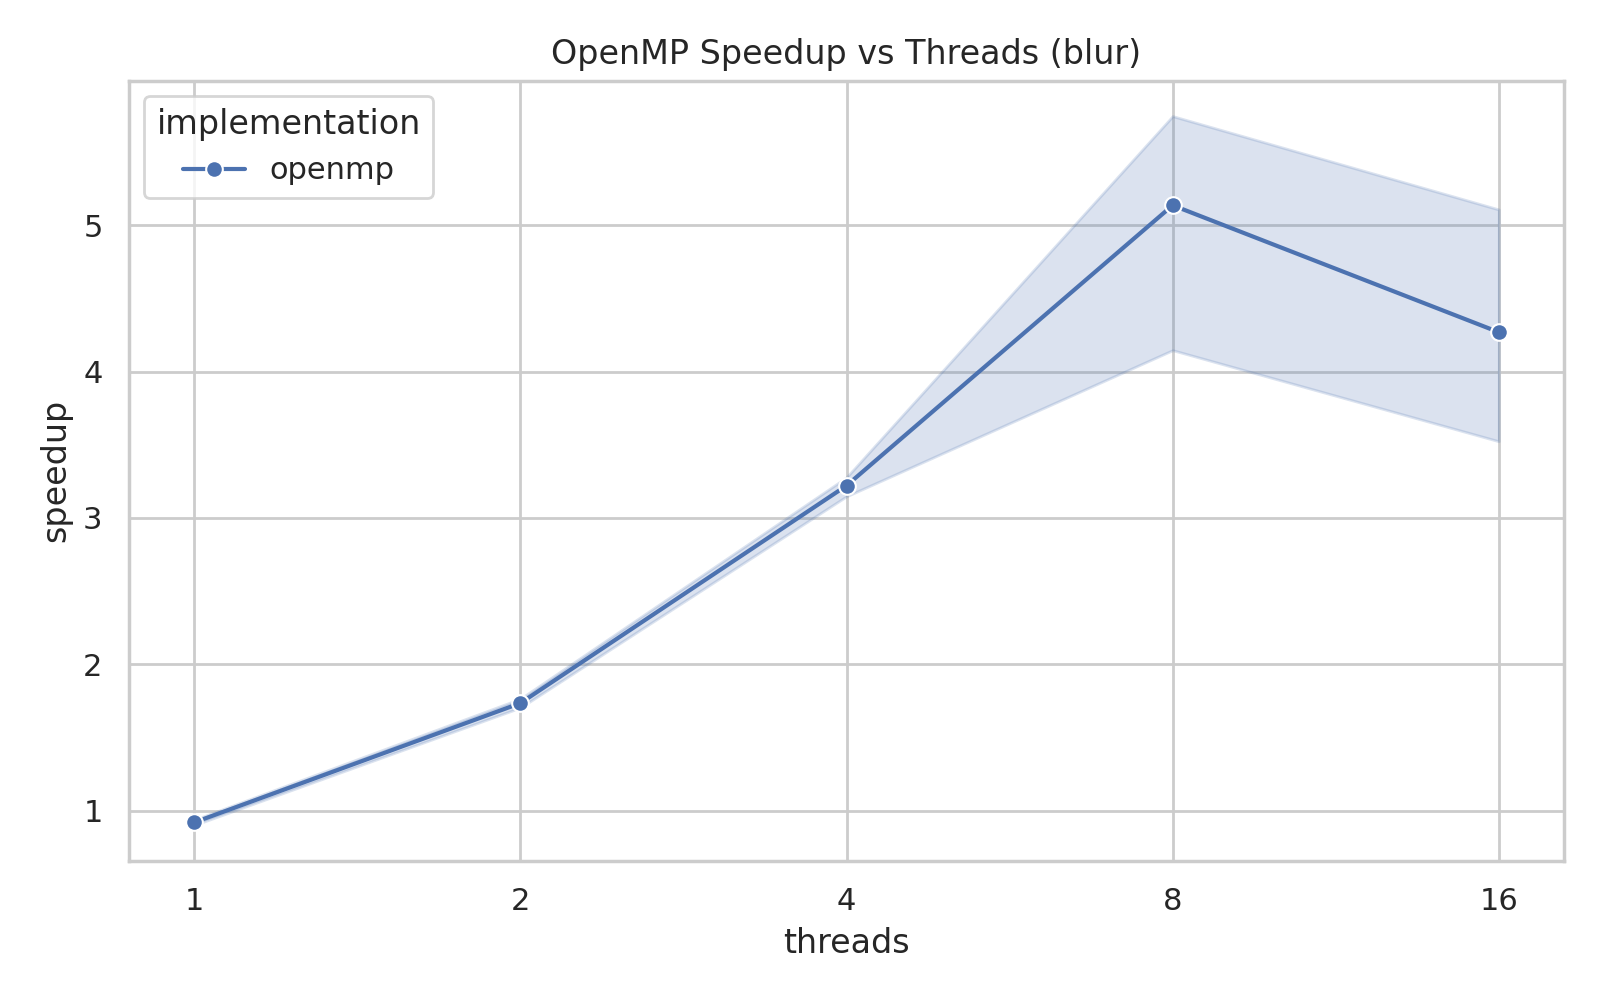
\includegraphics[keepaspectratio,alt={OpenMP speedup (blur)}]{./plots/output/openmp_speedup_blur.png}}
\pandocbounded{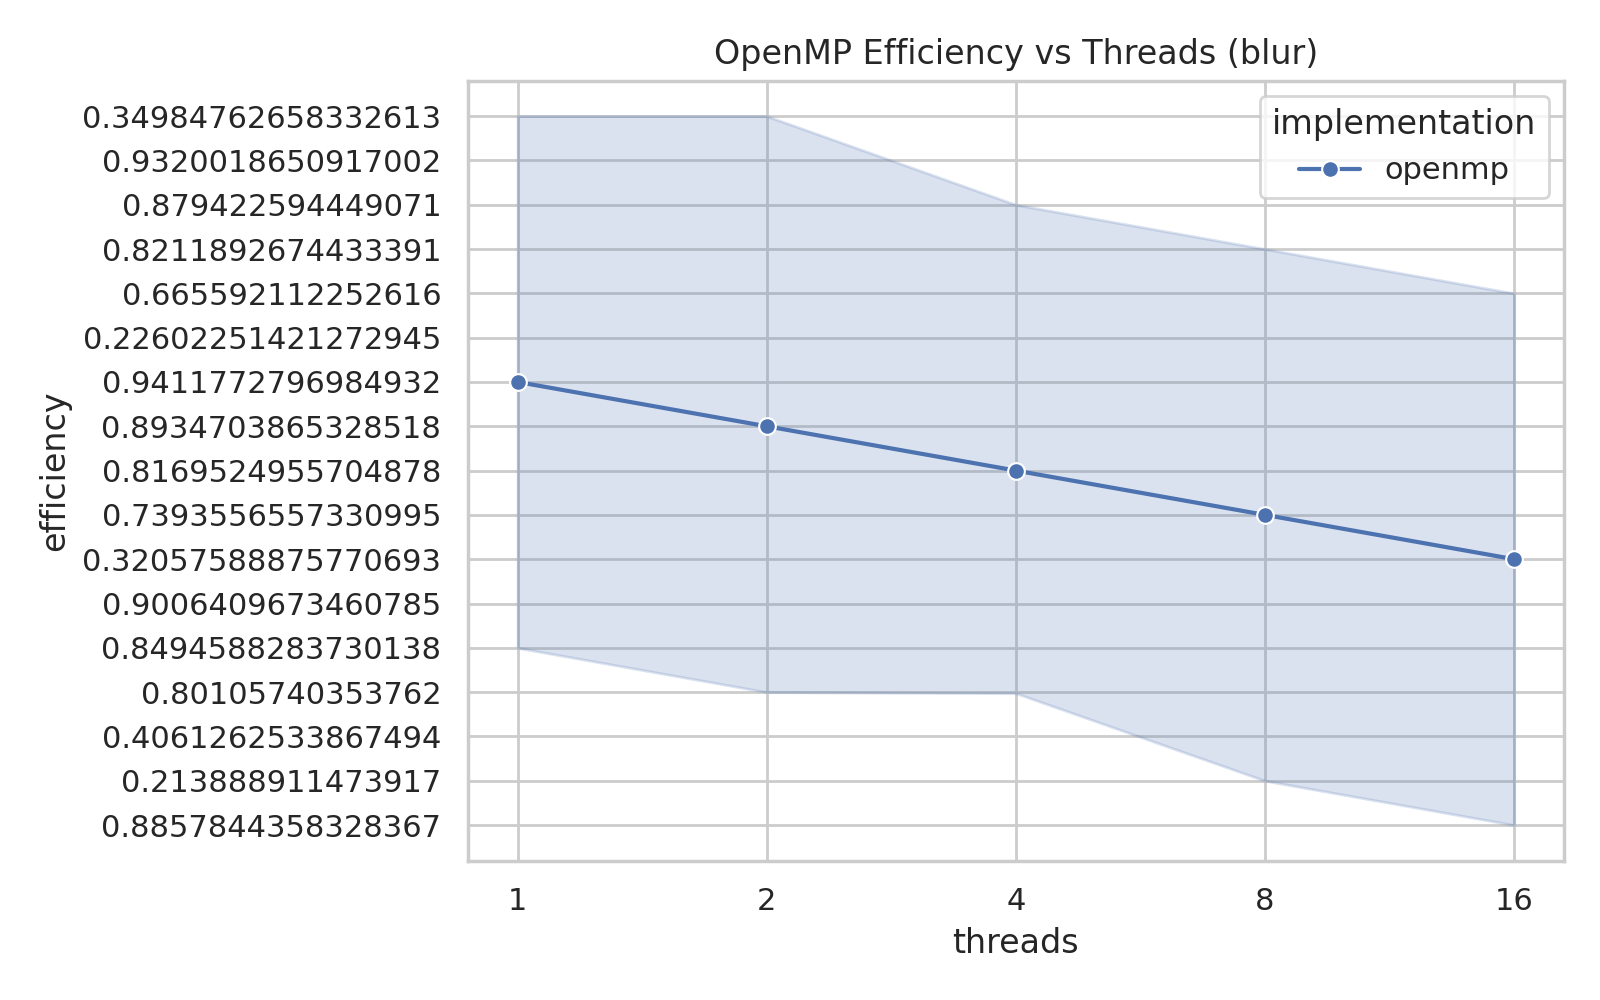
\includegraphics[keepaspectratio,alt={OpenMP efficiency (blur)}]{./plots/output/openmp_efficiency_blur.png}}

\pandocbounded{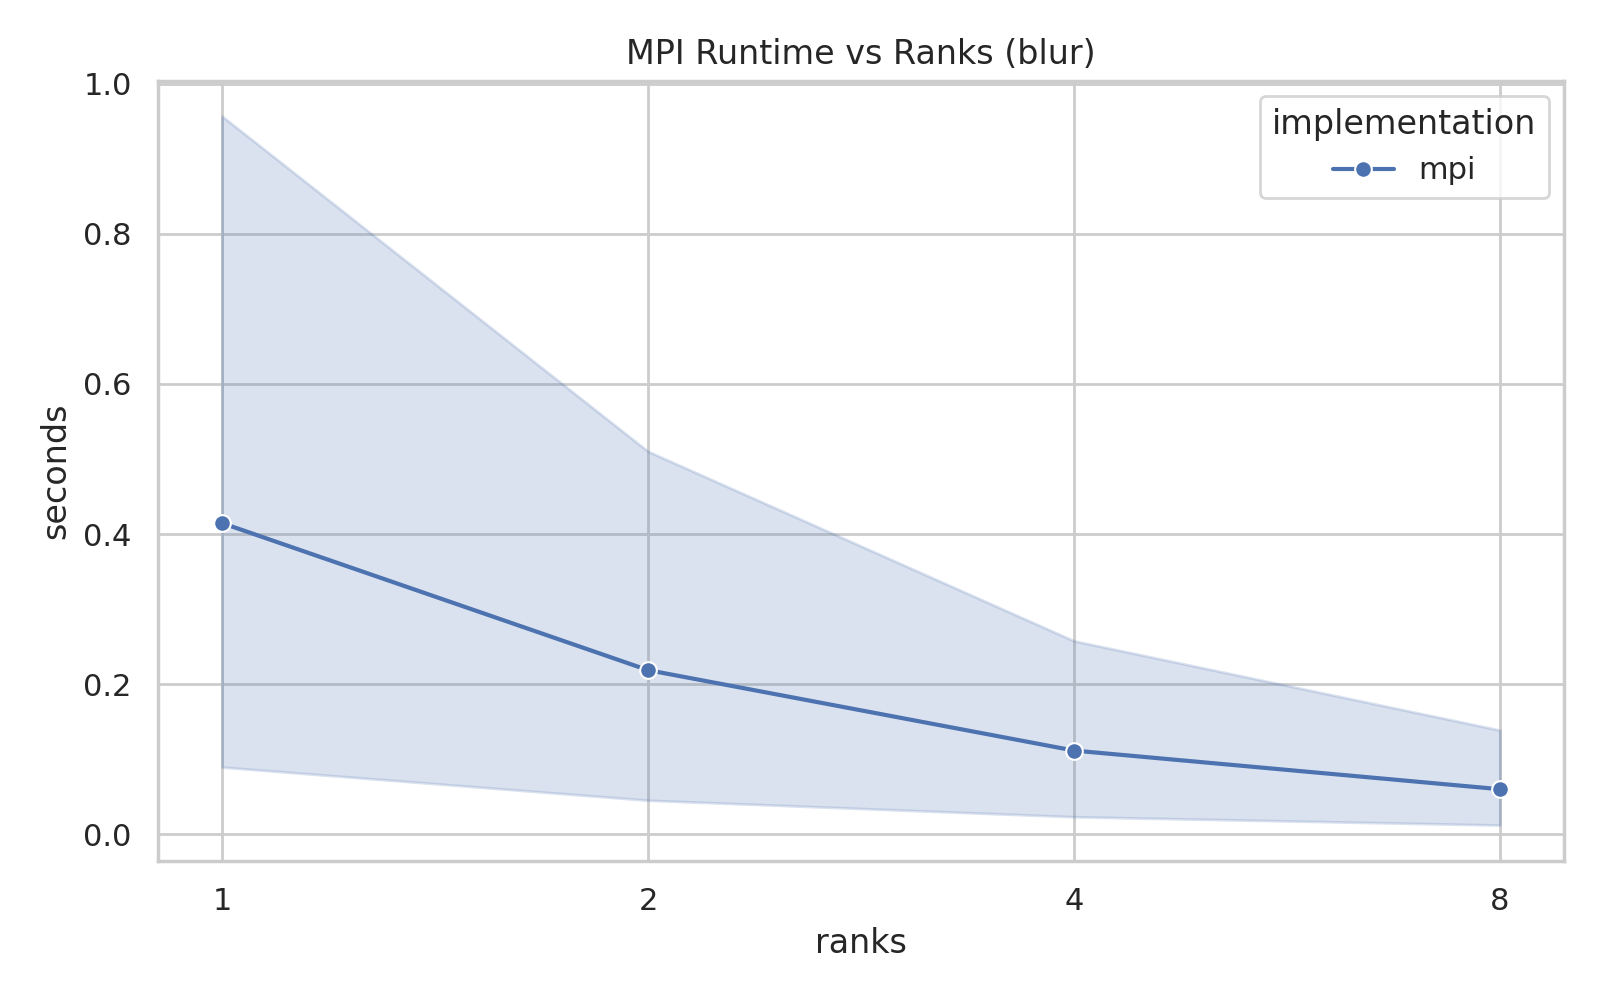
\includegraphics[keepaspectratio,alt={MPI runtime (blur)}]{./plots/output/mpi_time_blur.png}}
\pandocbounded{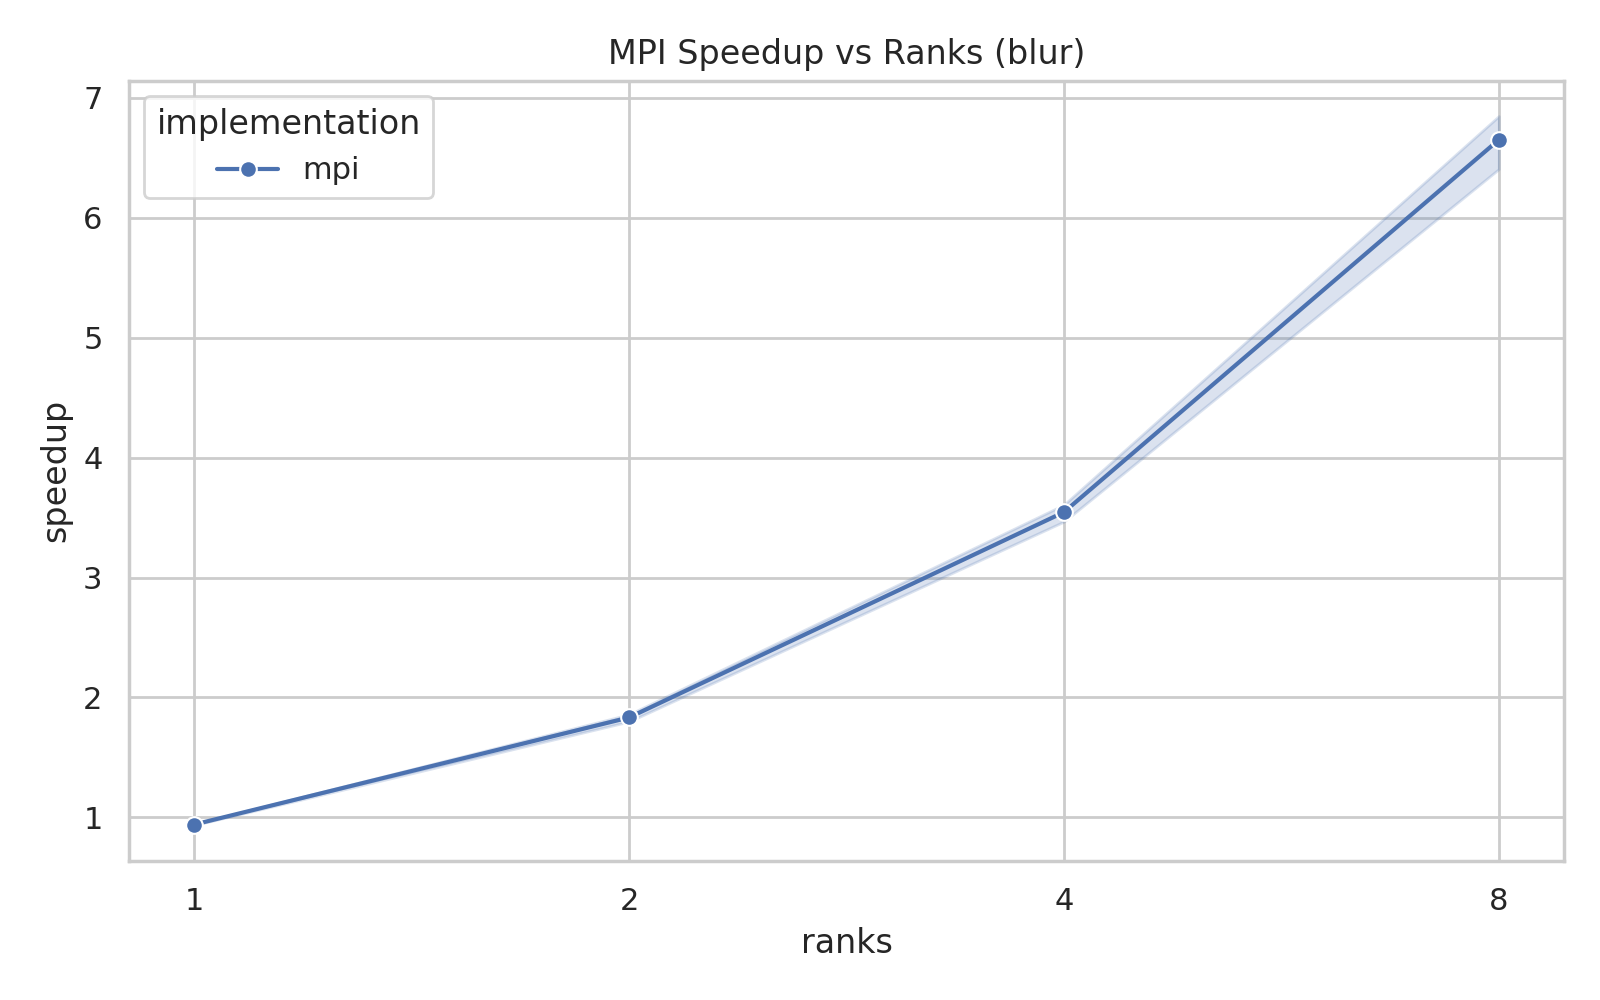
\includegraphics[keepaspectratio,alt={MPI speedup (blur)}]{./plots/output/mpi_speedup_blur.png}}
\pandocbounded{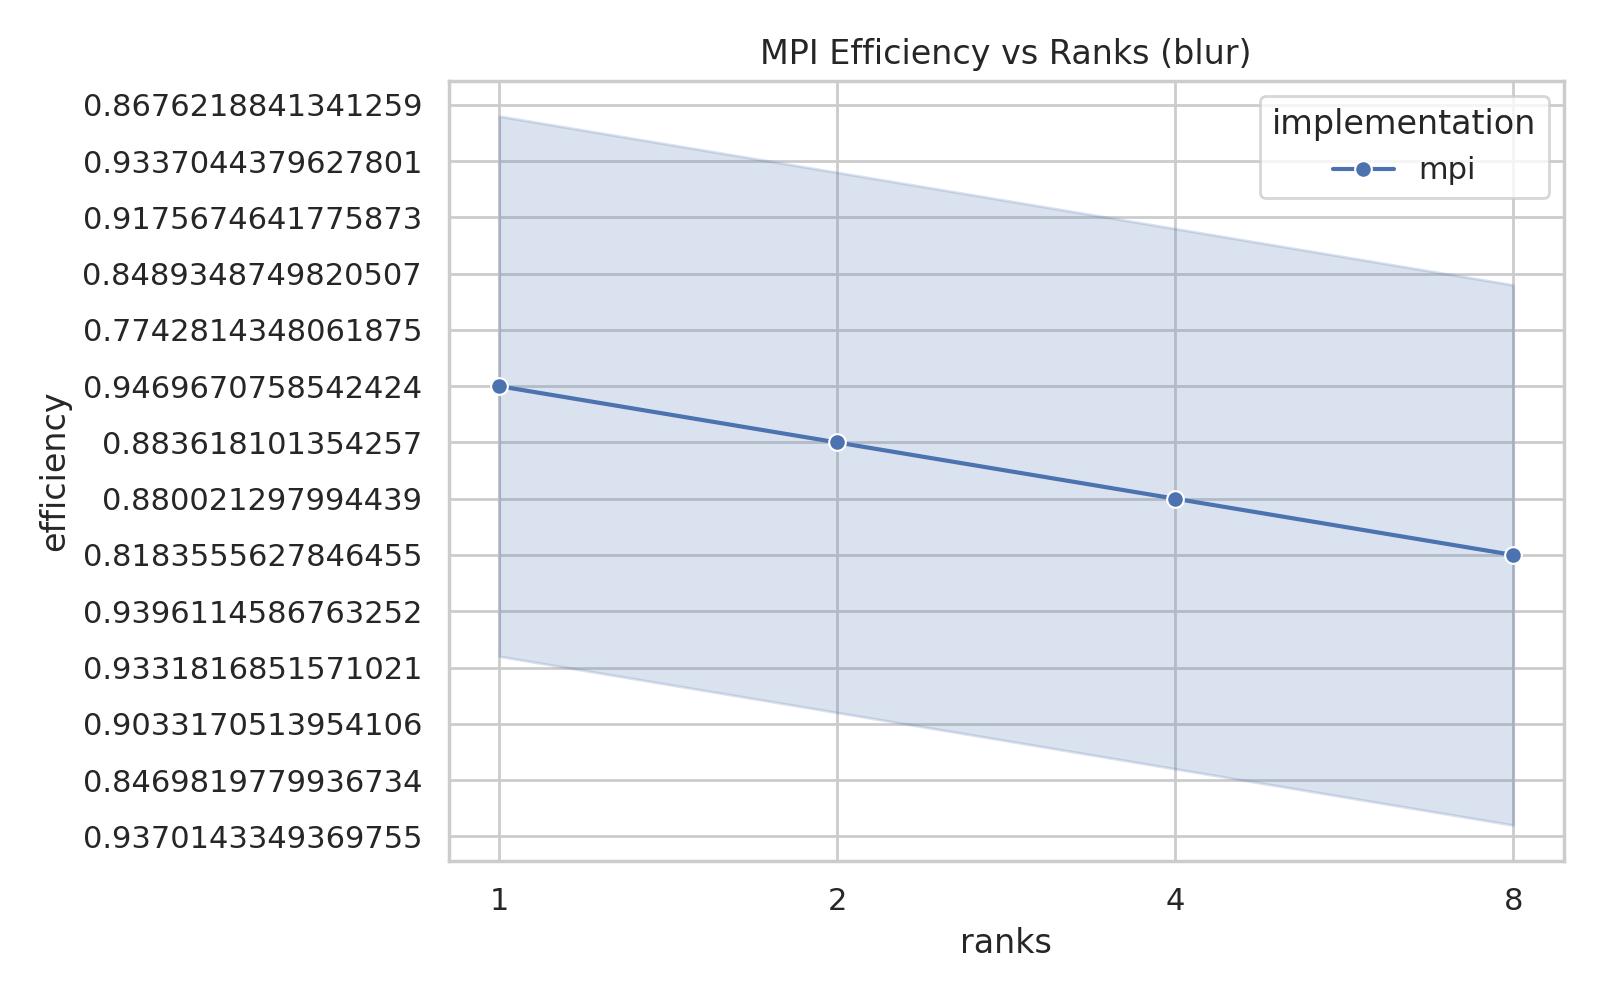
\includegraphics[keepaspectratio,alt={MPI efficiency (blur)}]{./plots/output/mpi_efficiency_blur.png}}

\pandocbounded{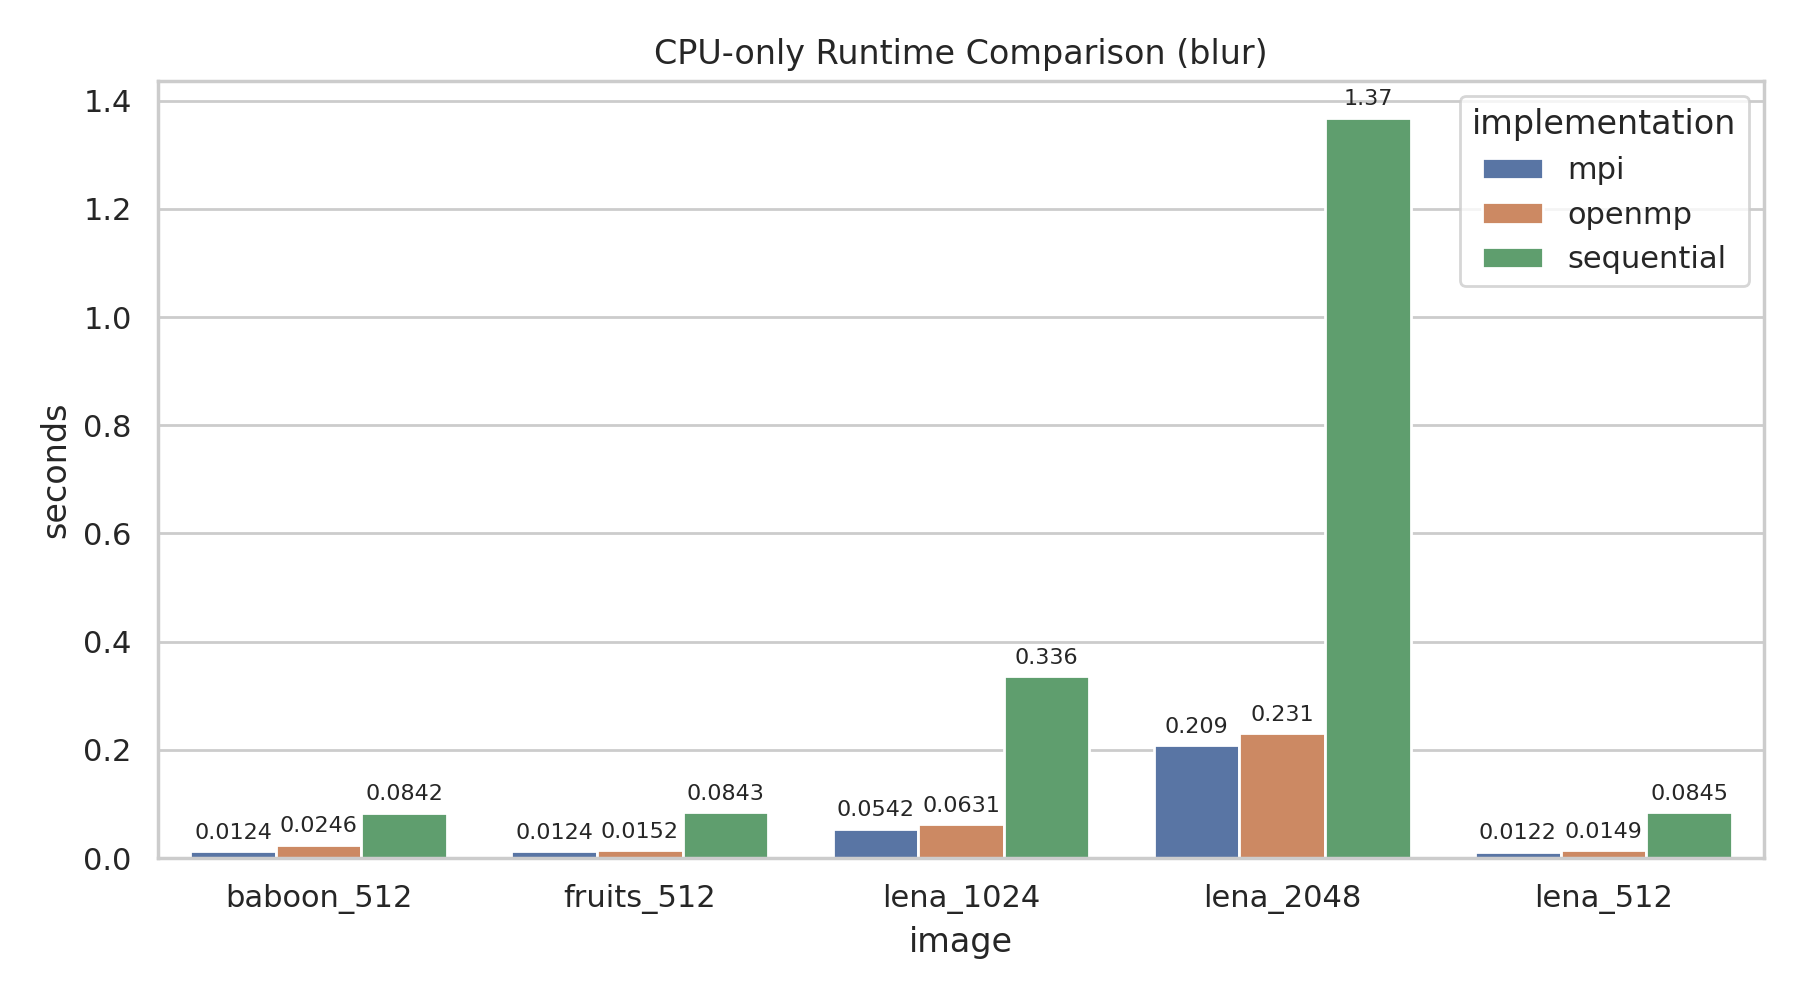
\includegraphics[keepaspectratio,alt={CPU-only runtime (blur)}]{./plots/output/cpu_only_runtime_blur.png}}
\pandocbounded{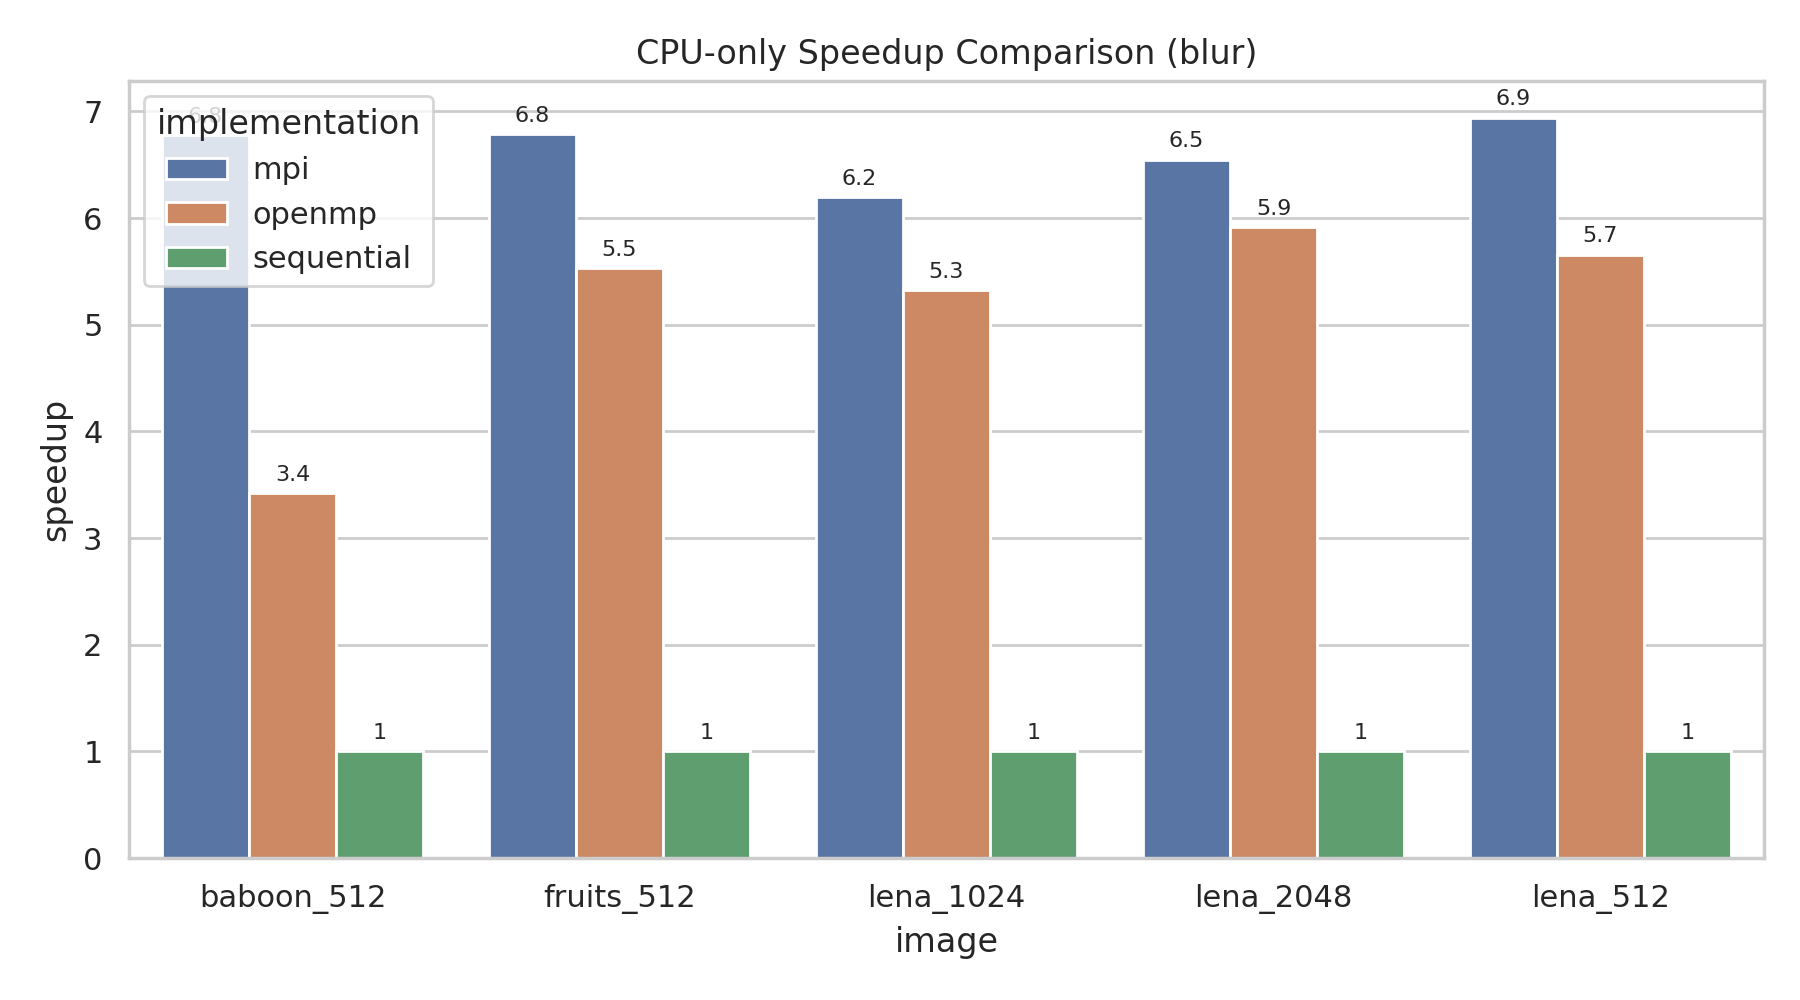
\includegraphics[keepaspectratio,alt={CPU-only speedup (blur)}]{./plots/output/cpu_only_speedup_blur.png}}

\pandocbounded{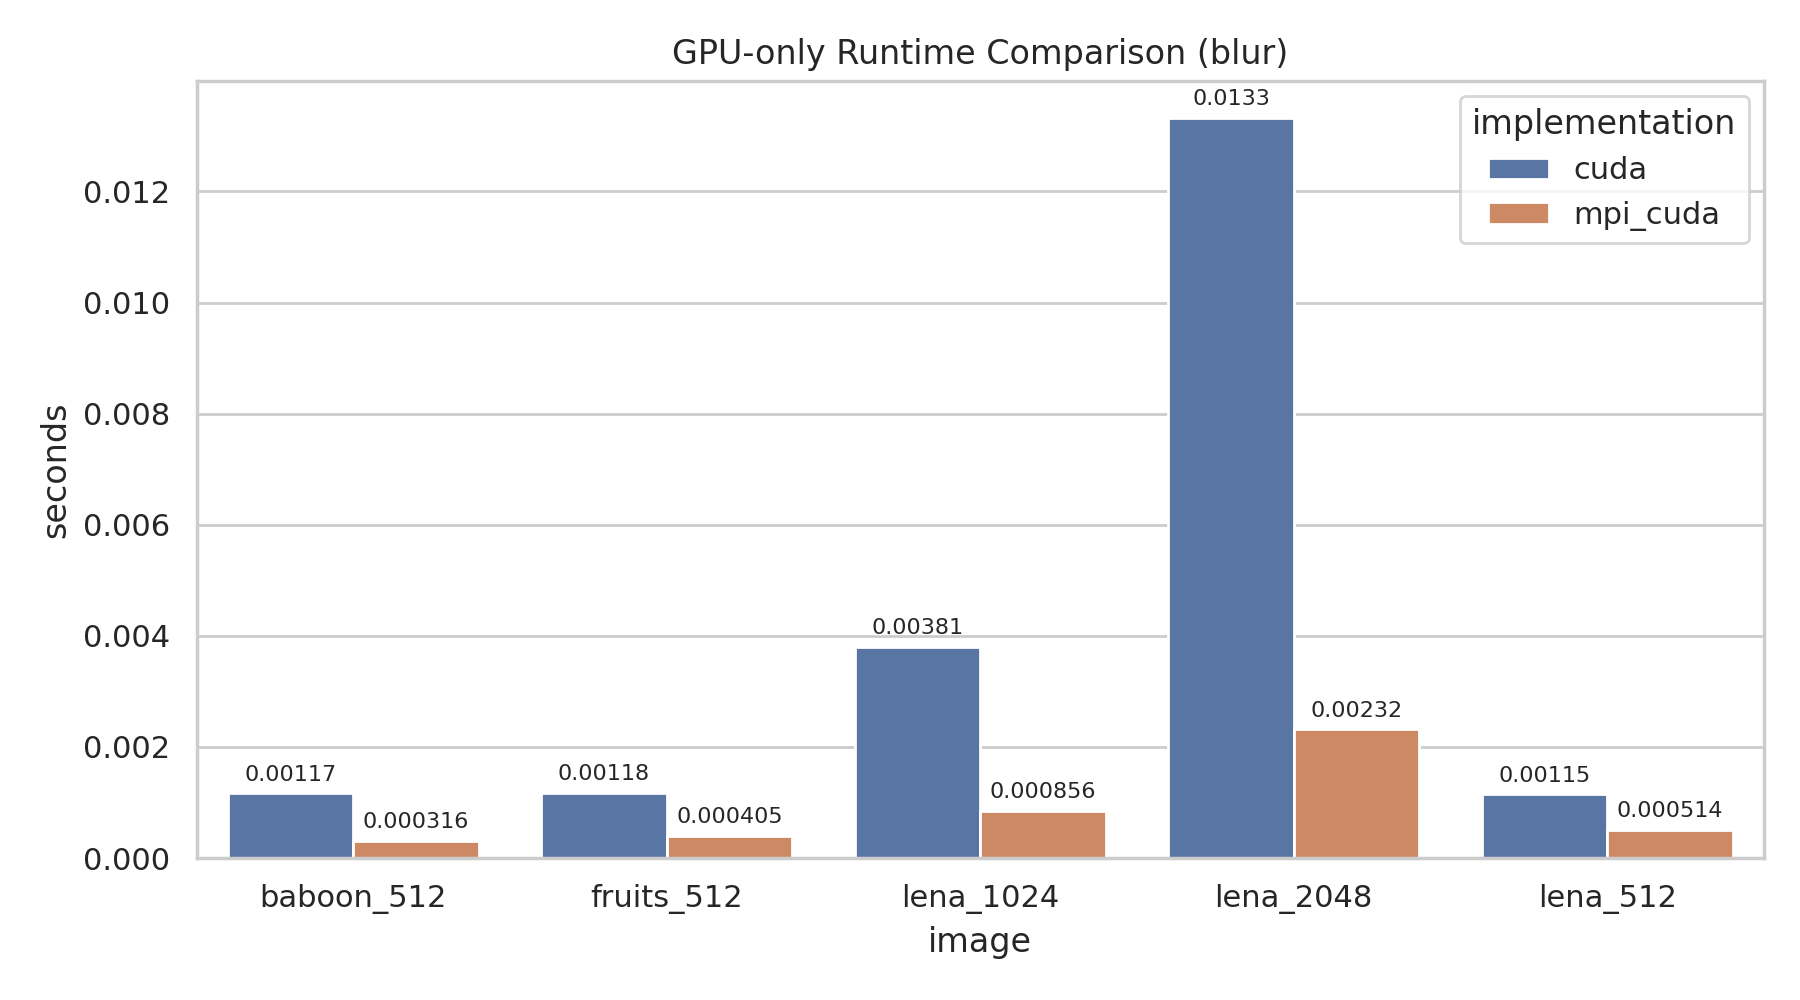
\includegraphics[keepaspectratio,alt={GPU-only runtime (blur)}]{./plots/output/gpu_only_runtime_blur.png}}
\pandocbounded{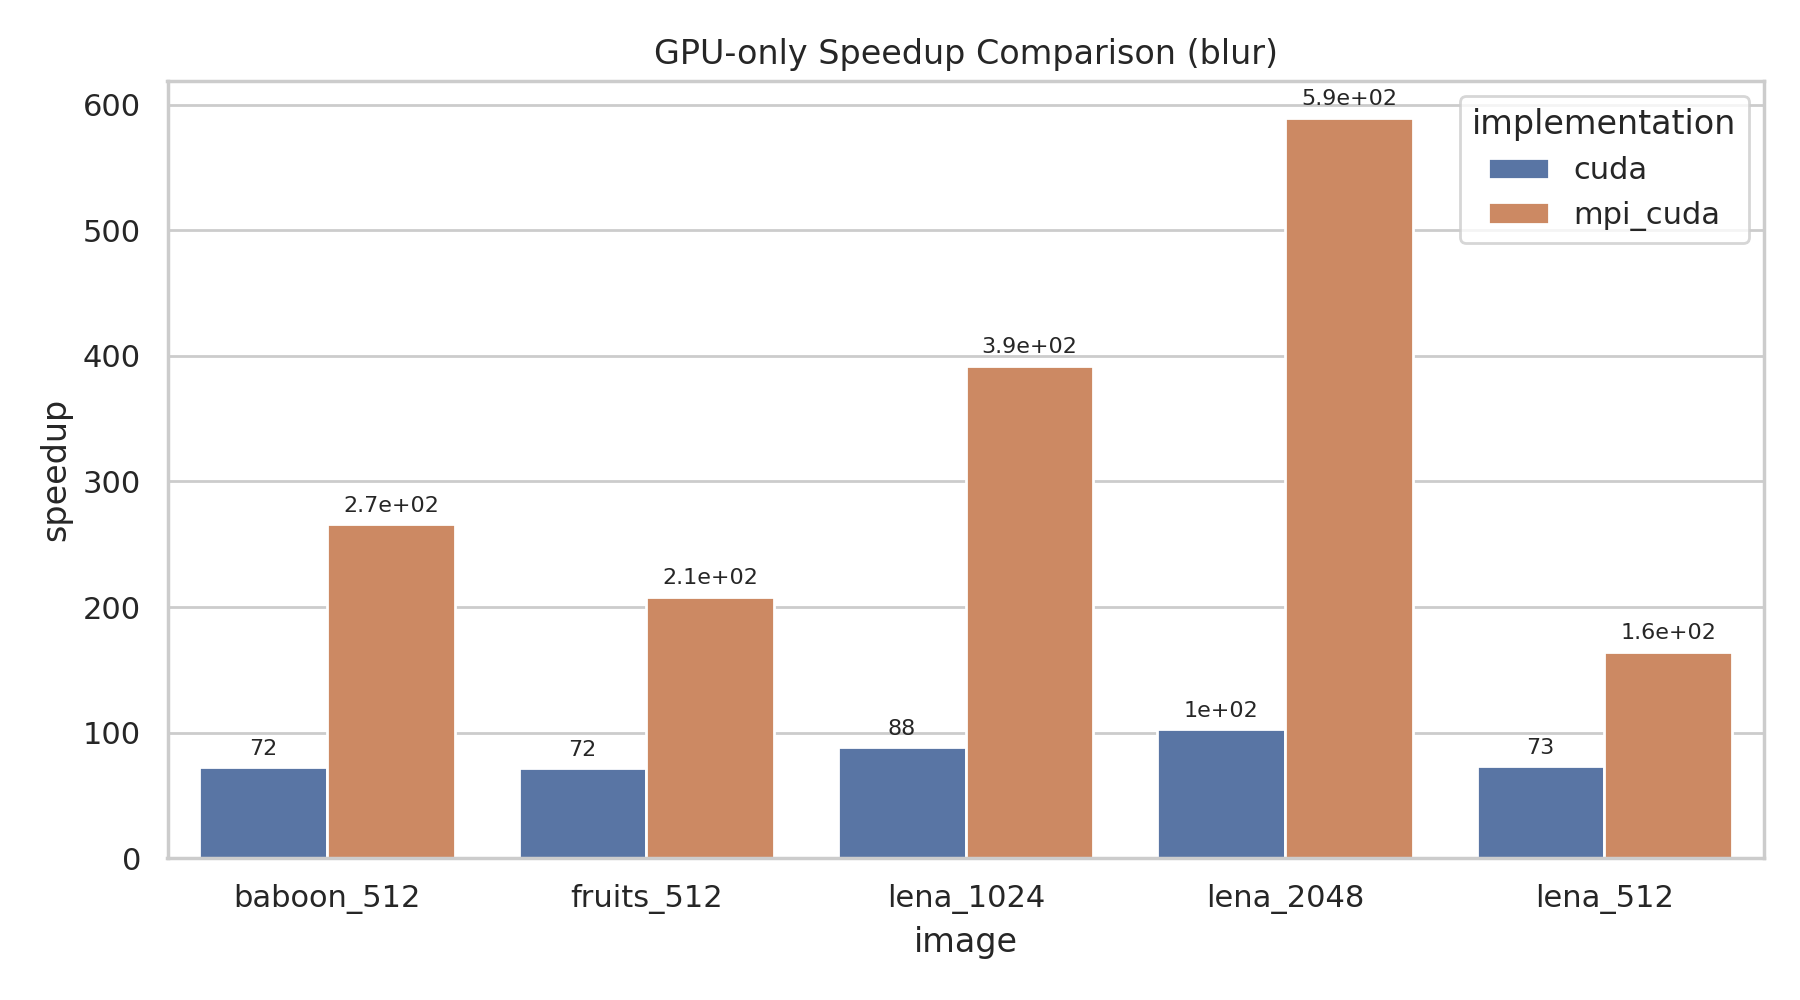
\includegraphics[keepaspectratio,alt={GPU-only speedup (blur)}]{./plots/output/gpu_only_speedup_blur.png}}

\pandocbounded{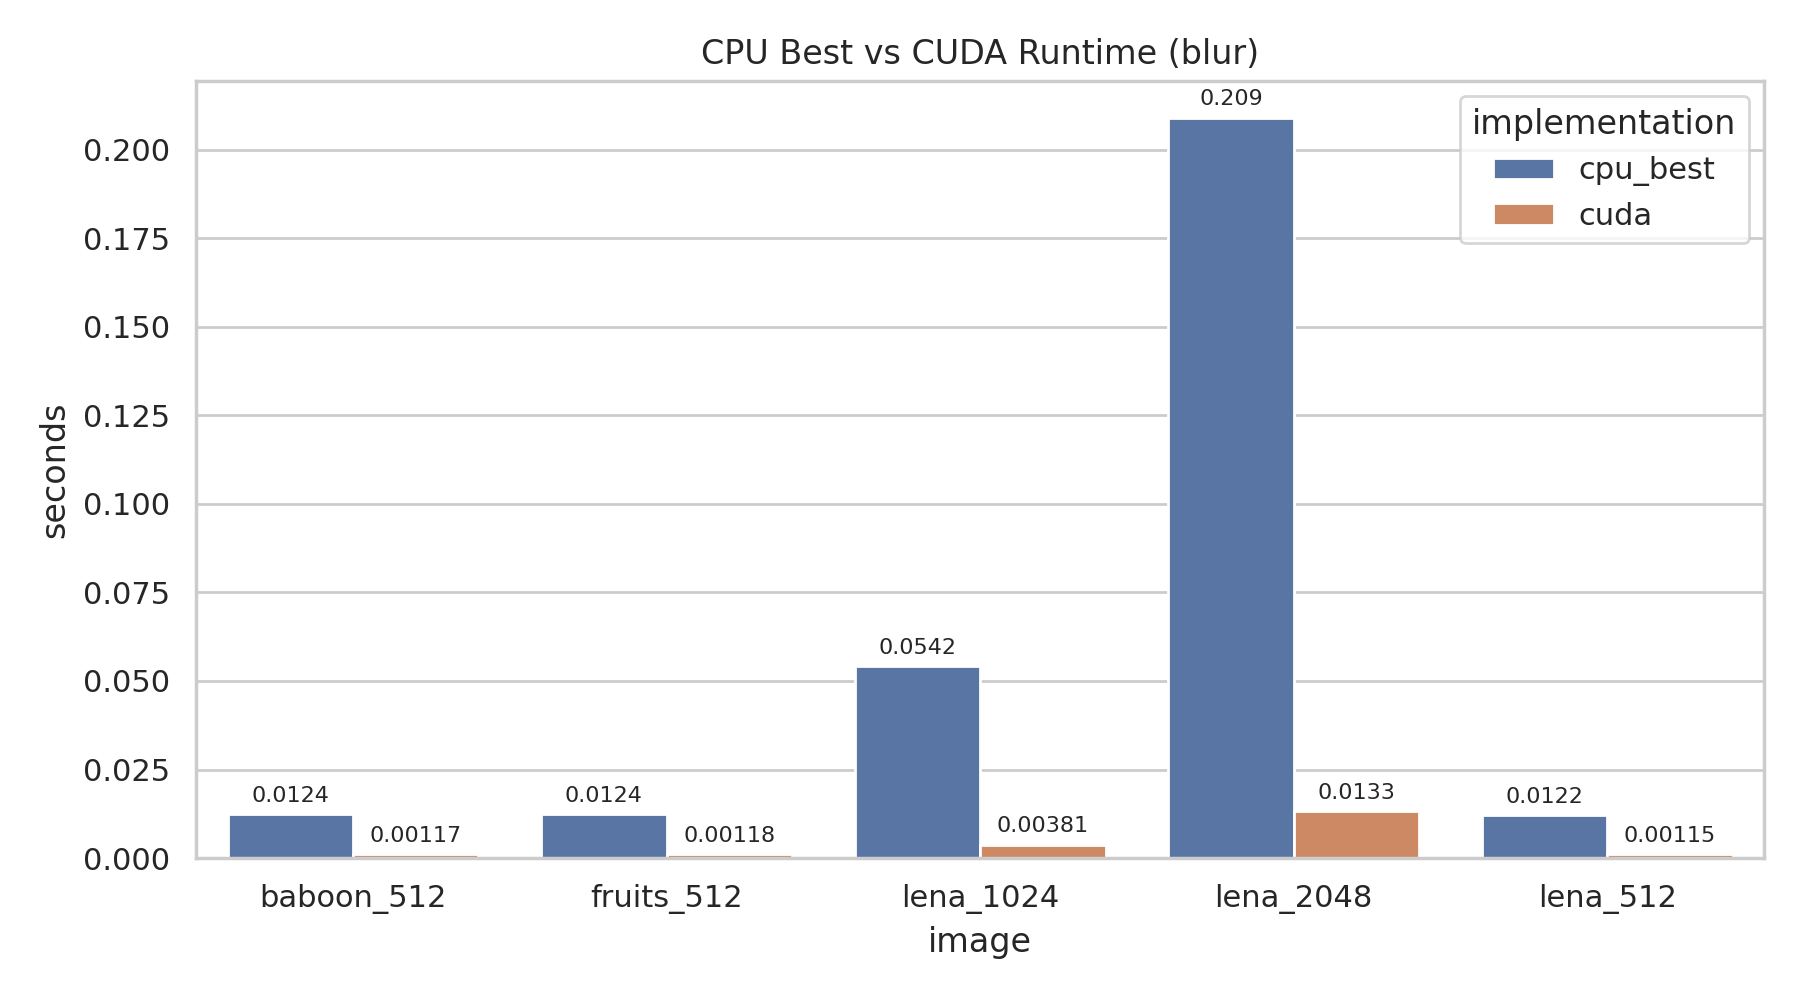
\includegraphics[keepaspectratio,alt={CPU vs CUDA runtime (blur)}]{./plots/output/cpu_vs_cuda_runtime_blur.png}}
\pandocbounded{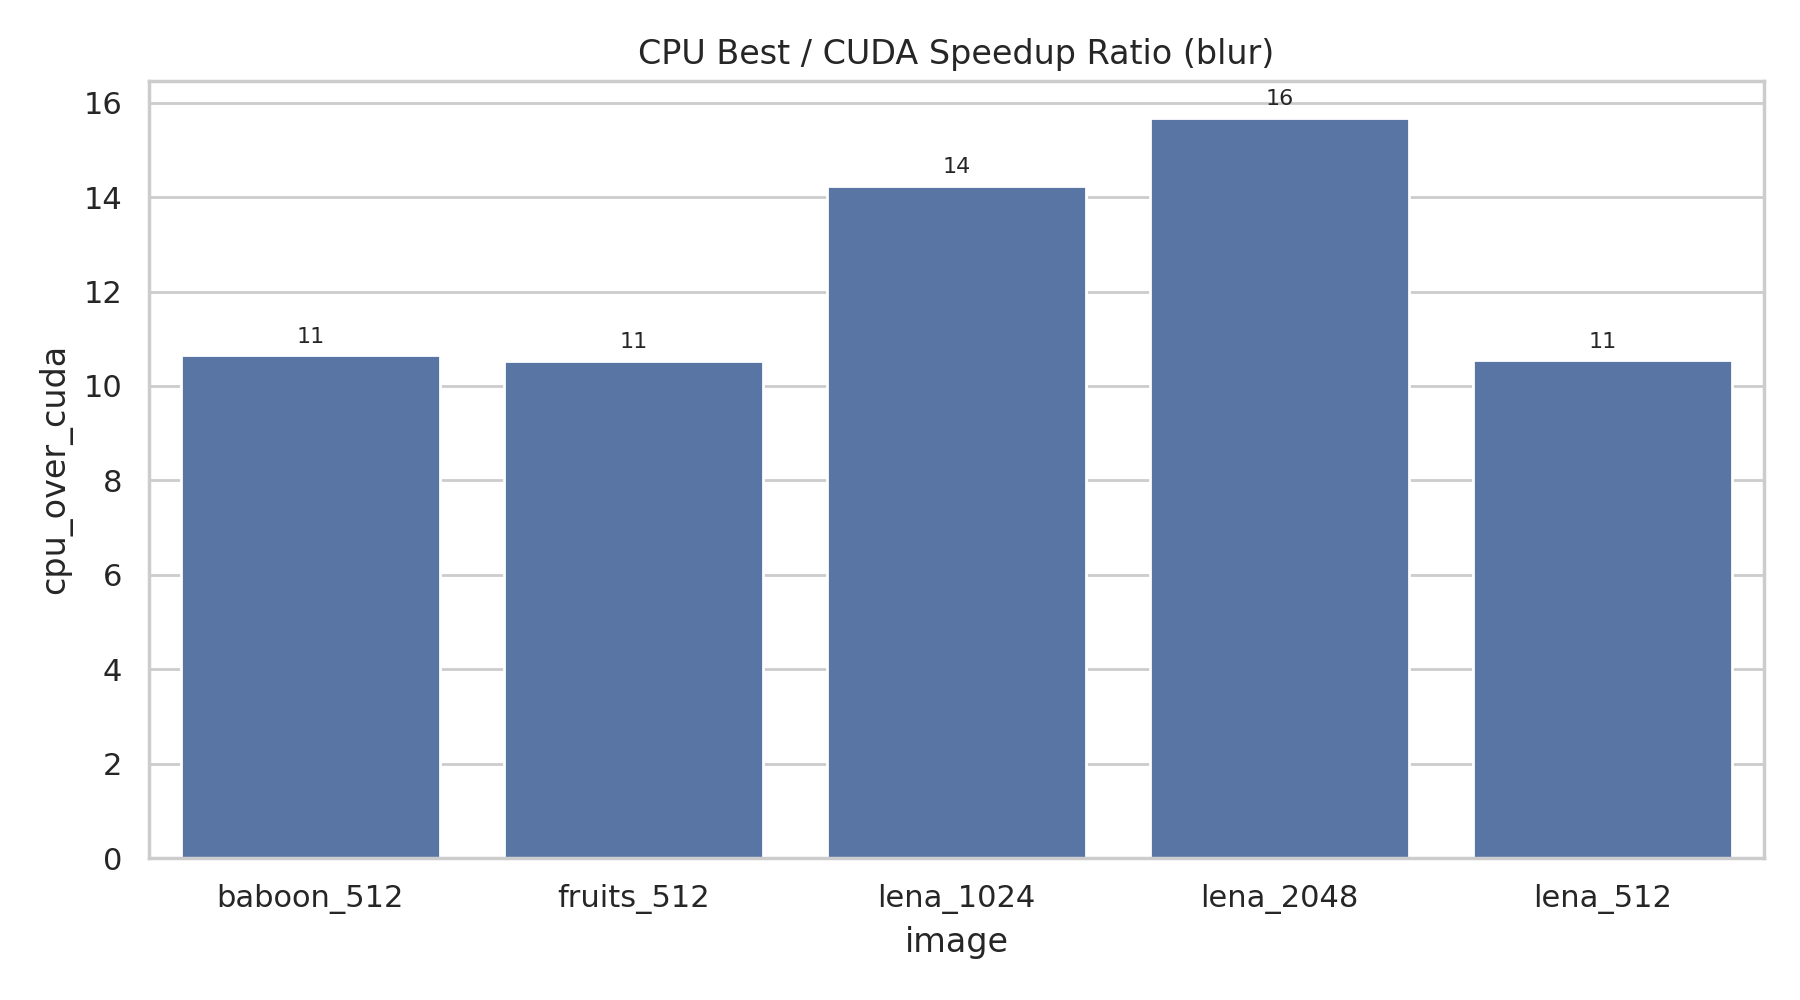
\includegraphics[keepaspectratio,alt={CPU vs CUDA speedup (blur)}]{./plots/output/cpu_vs_cuda_speedup_blur.png}}

\pandocbounded{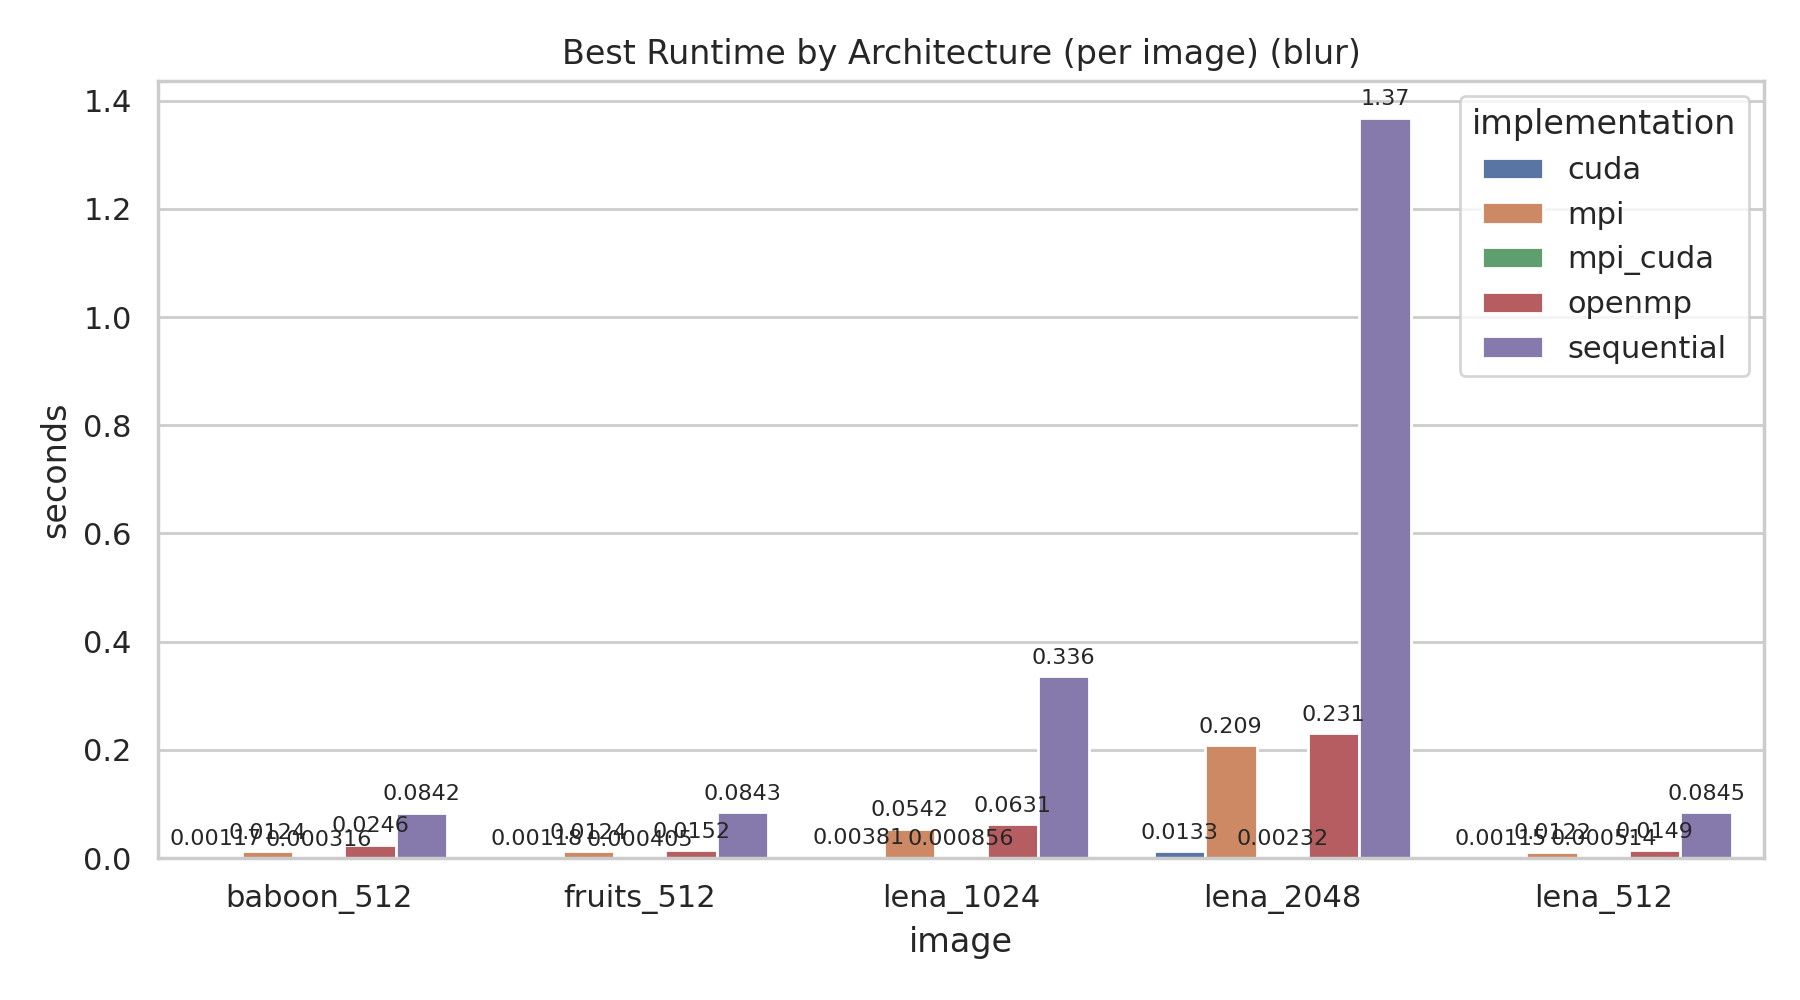
\includegraphics[keepaspectratio,alt={Cross-architecture runtime comparison (blur)}]{./plots/output/arch_time_comparison_blur.png}}
\pandocbounded{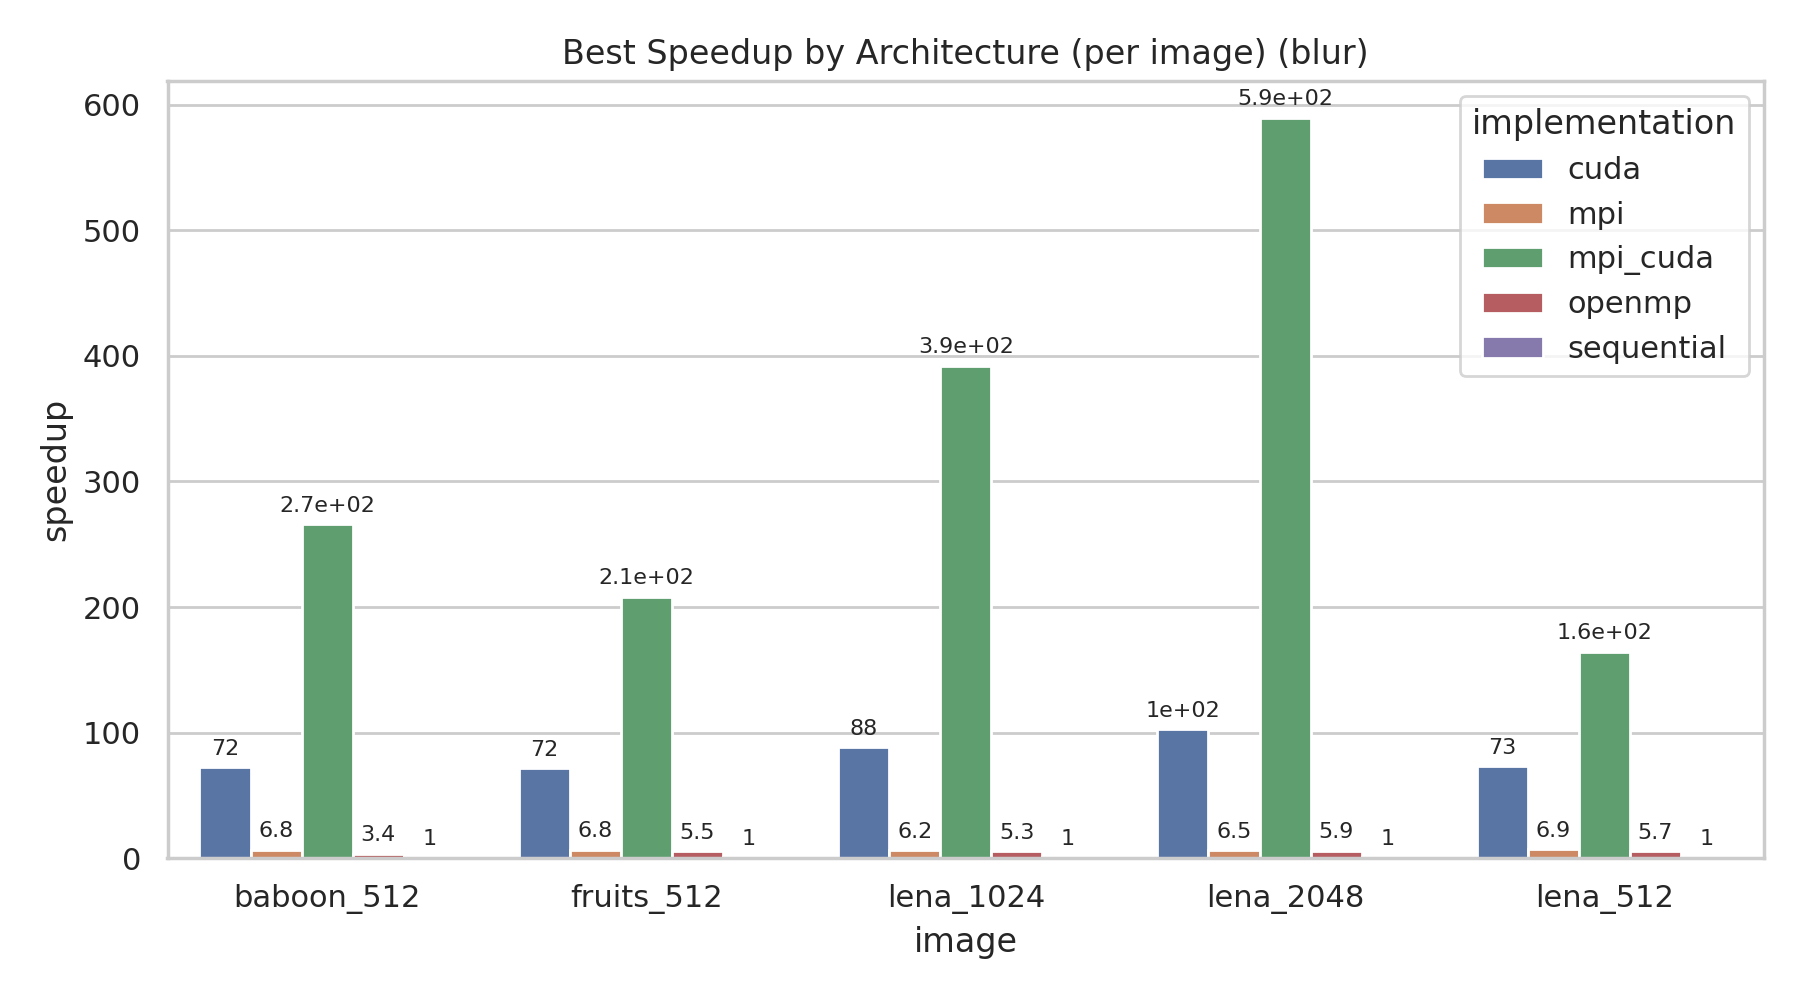
\includegraphics[keepaspectratio,alt={Cross-architecture speedup comparison (blur)}]{./plots/output/arch_speedup_comparison_blur.png}}

\textbf{Sobel (3 x 3)}

\pandocbounded{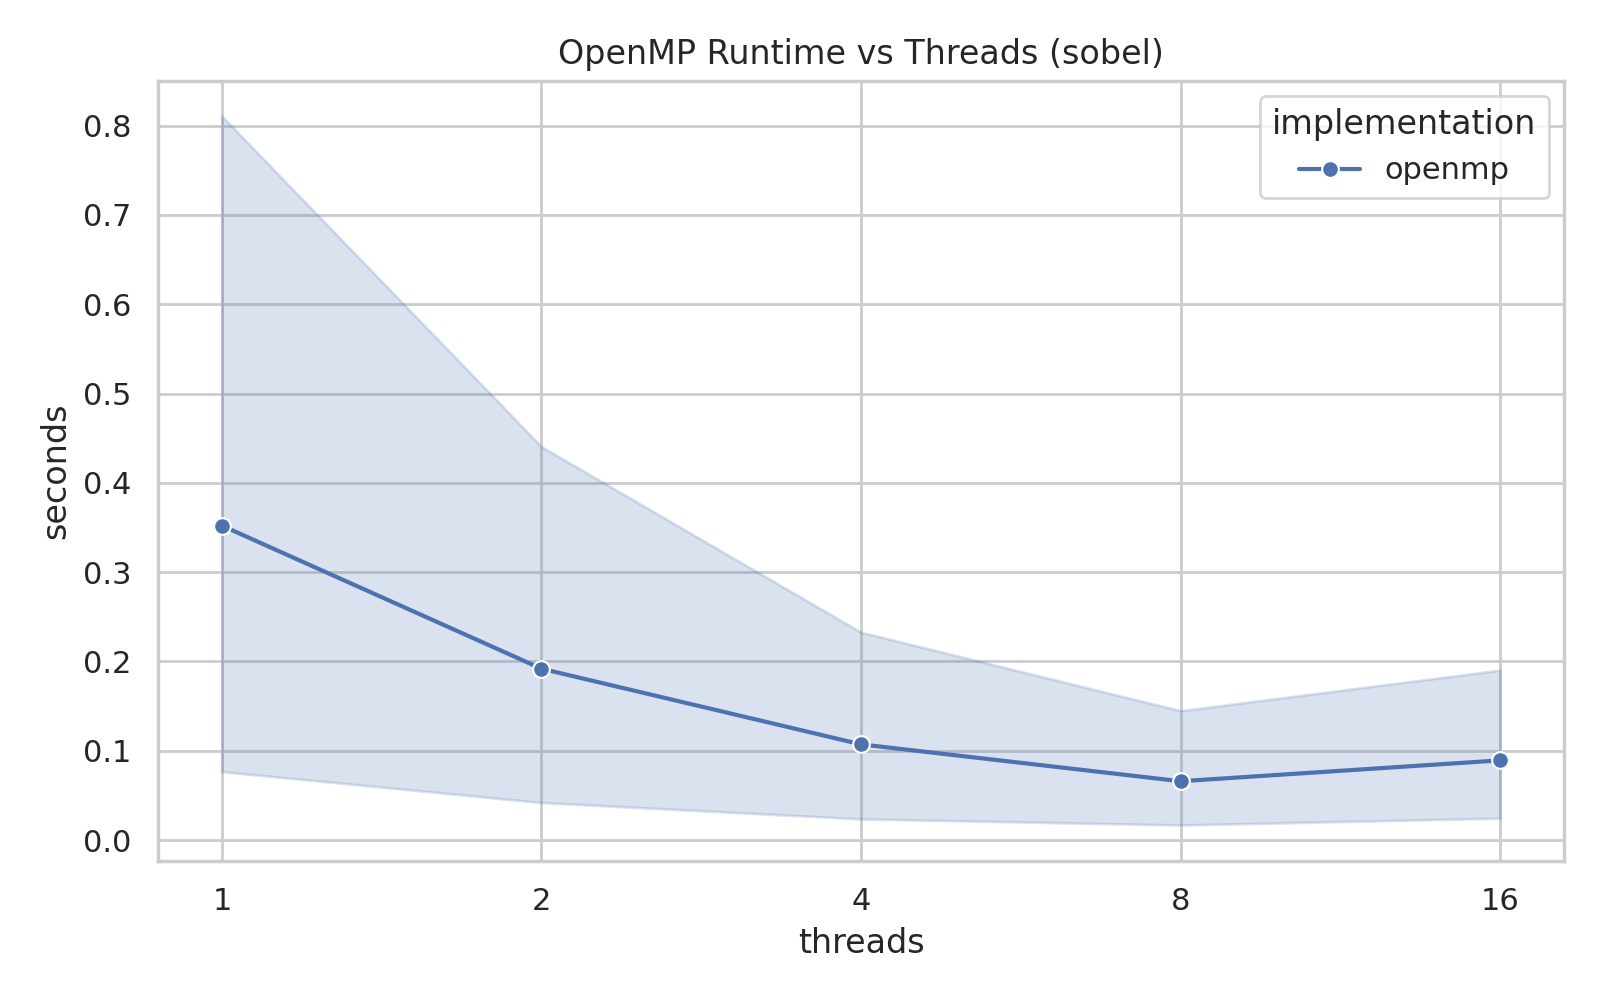
\includegraphics[keepaspectratio,alt={OpenMP runtime (sobel)}]{./plots/output/openmp_time_sobel.png}}
\pandocbounded{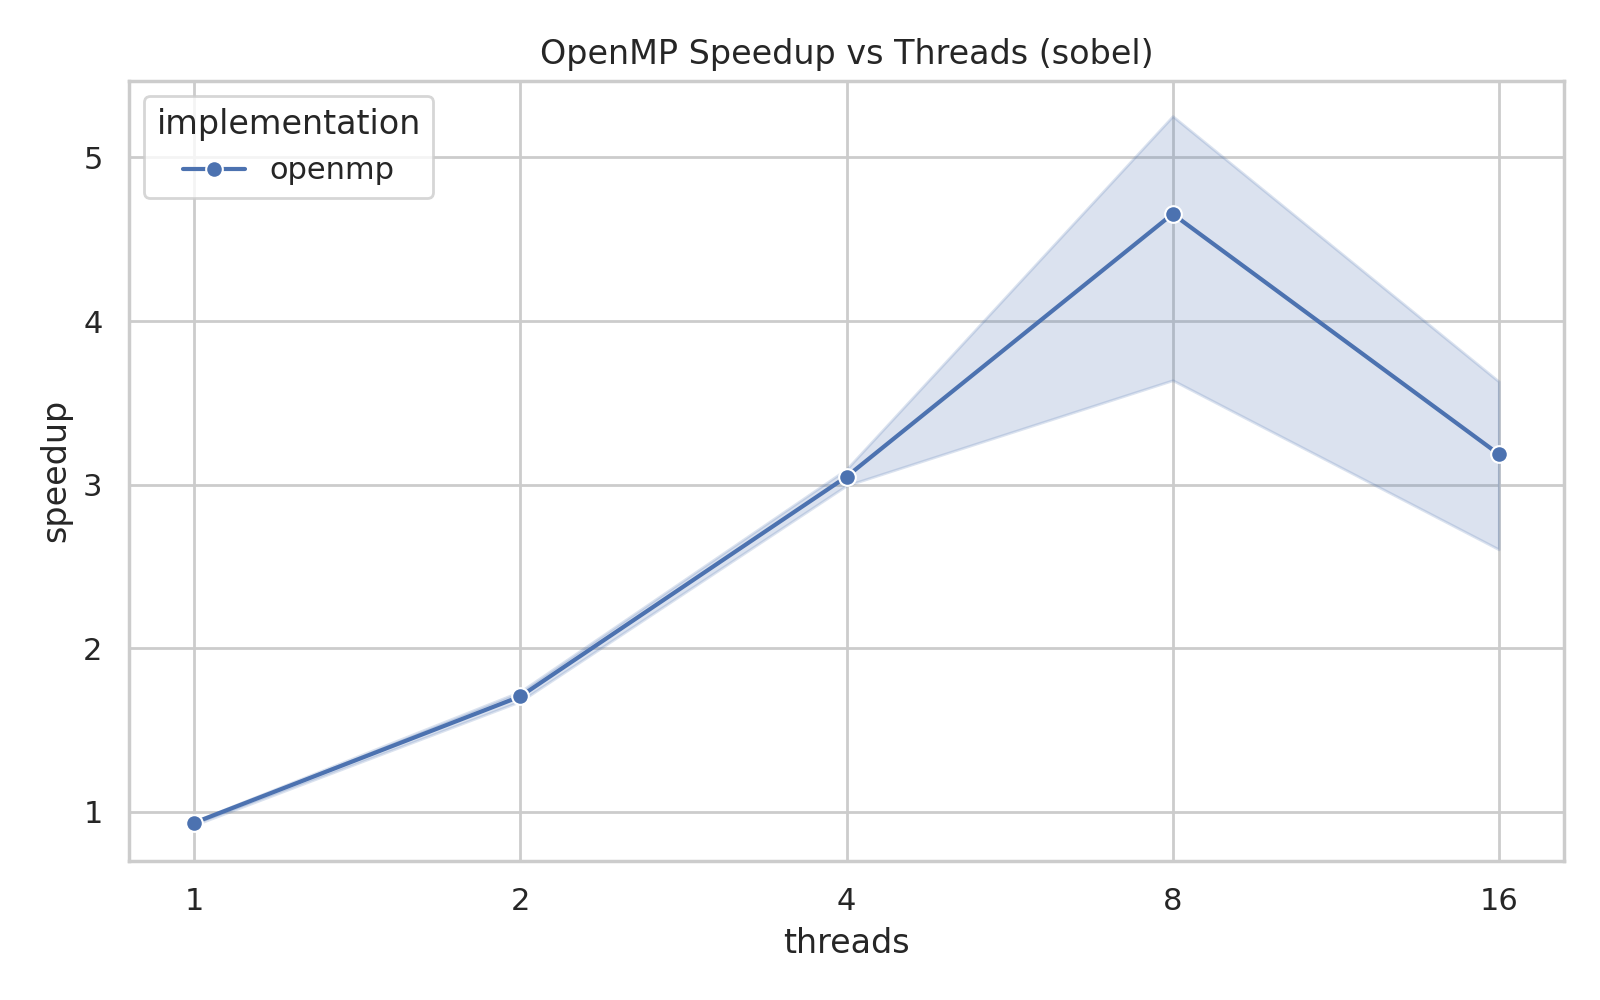
\includegraphics[keepaspectratio,alt={OpenMP speedup (sobel)}]{./plots/output/openmp_speedup_sobel.png}}
\pandocbounded{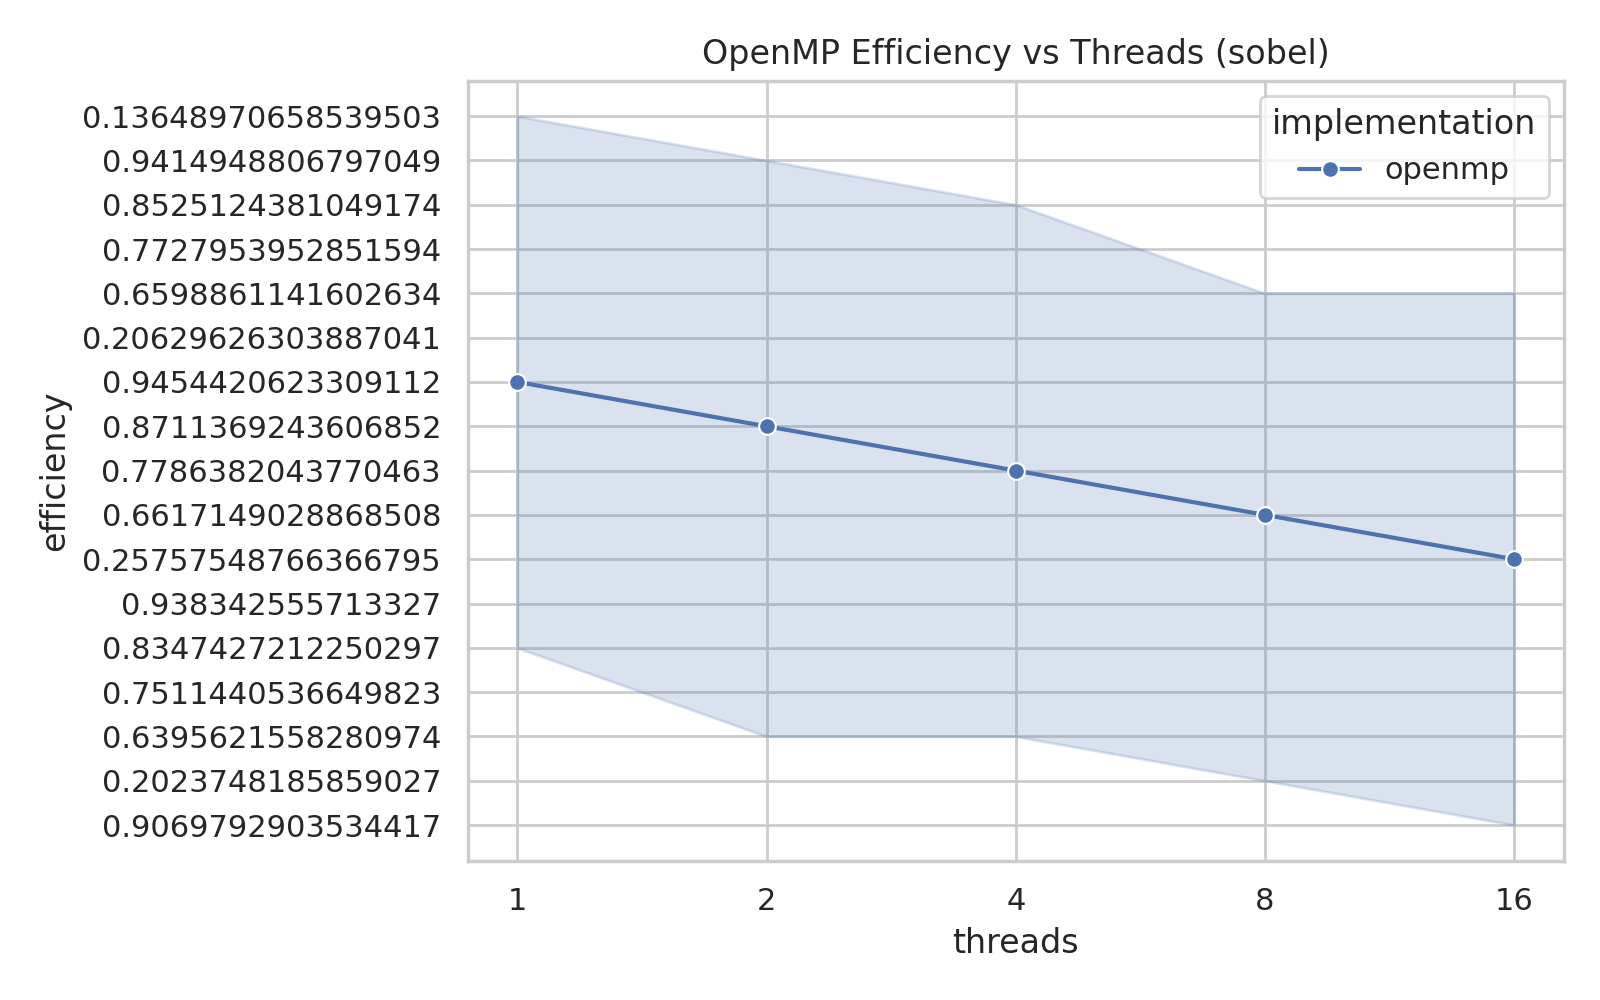
\includegraphics[keepaspectratio,alt={OpenMP efficiency (sobel)}]{./plots/output/openmp_efficiency_sobel.png}}

\pandocbounded{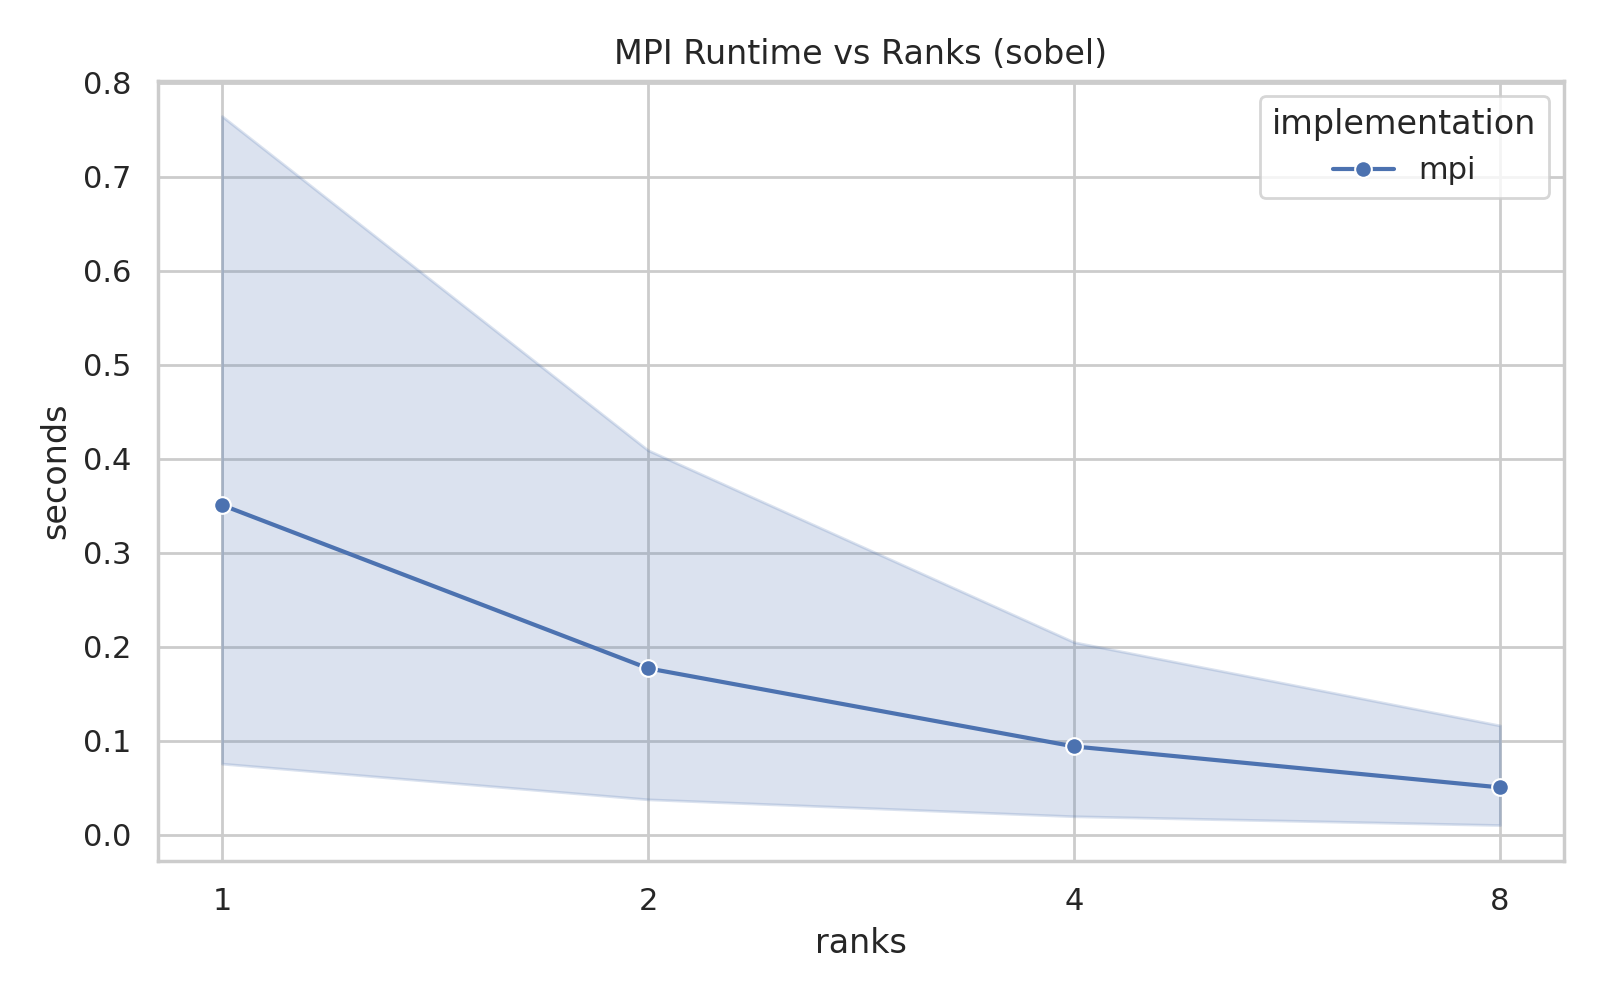
\includegraphics[keepaspectratio,alt={MPI runtime (sobel)}]{./plots/output/mpi_time_sobel.png}}
\pandocbounded{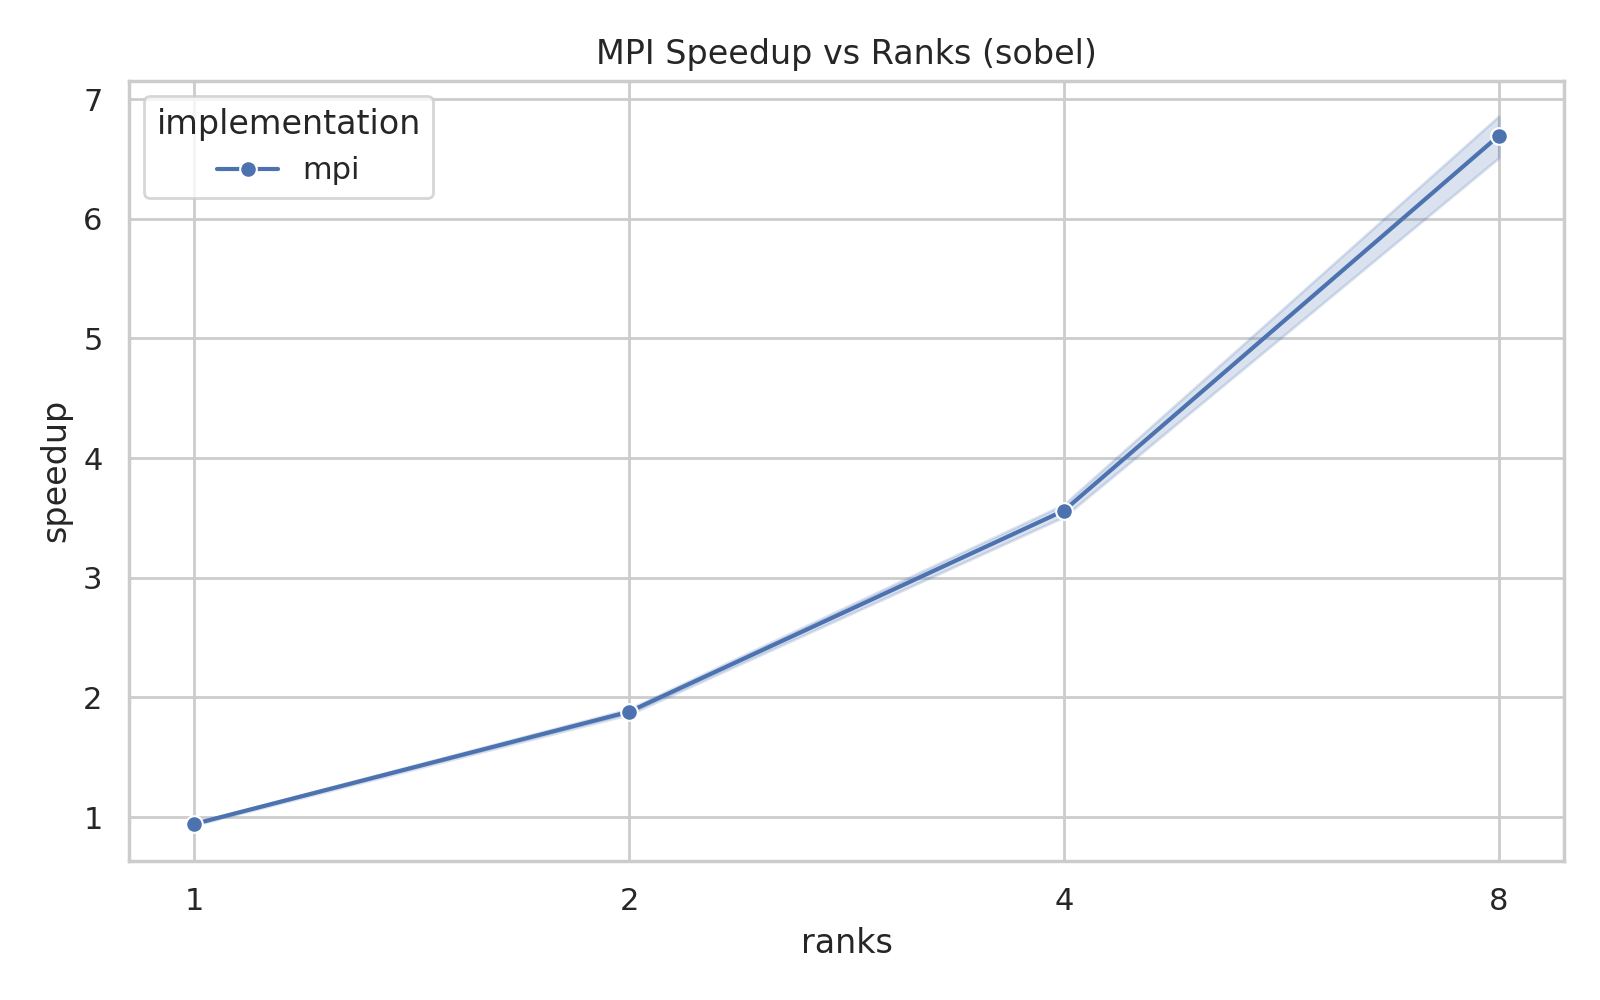
\includegraphics[keepaspectratio,alt={MPI speedup (sobel)}]{./plots/output/mpi_speedup_sobel.png}}
\pandocbounded{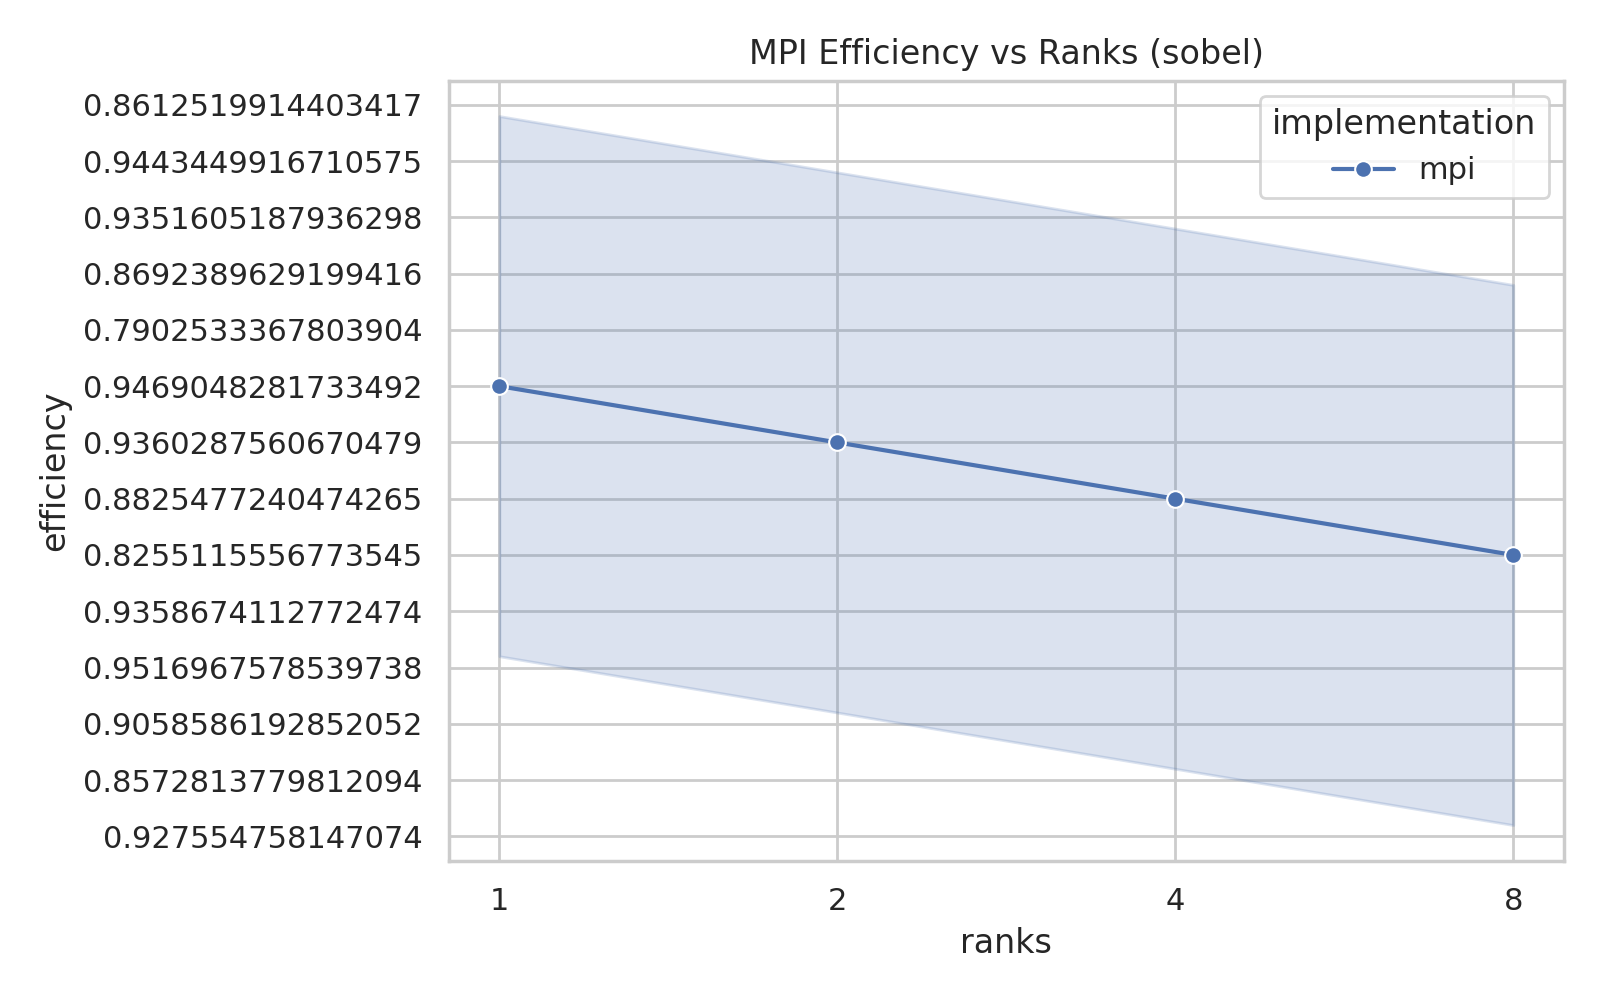
\includegraphics[keepaspectratio,alt={MPI efficiency (sobel)}]{./plots/output/mpi_efficiency_sobel.png}}

\pandocbounded{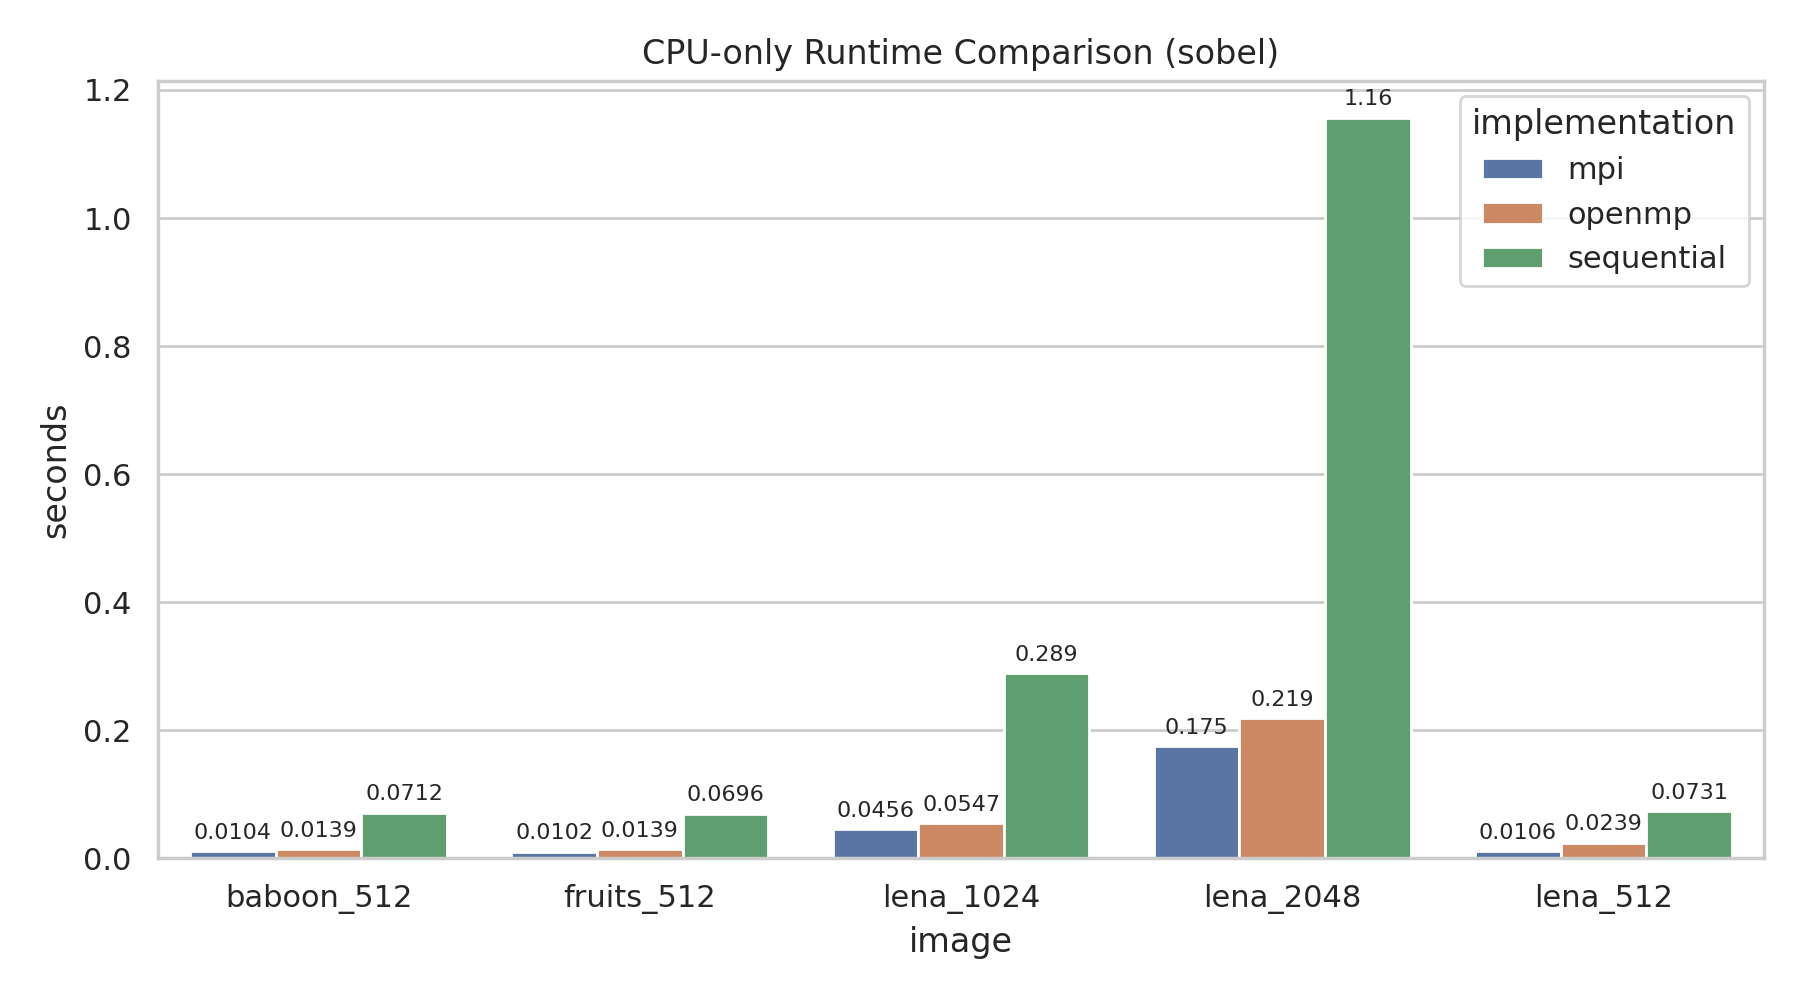
\includegraphics[keepaspectratio,alt={CPU-only runtime (sobel)}]{./plots/output/cpu_only_runtime_sobel.png}}
\pandocbounded{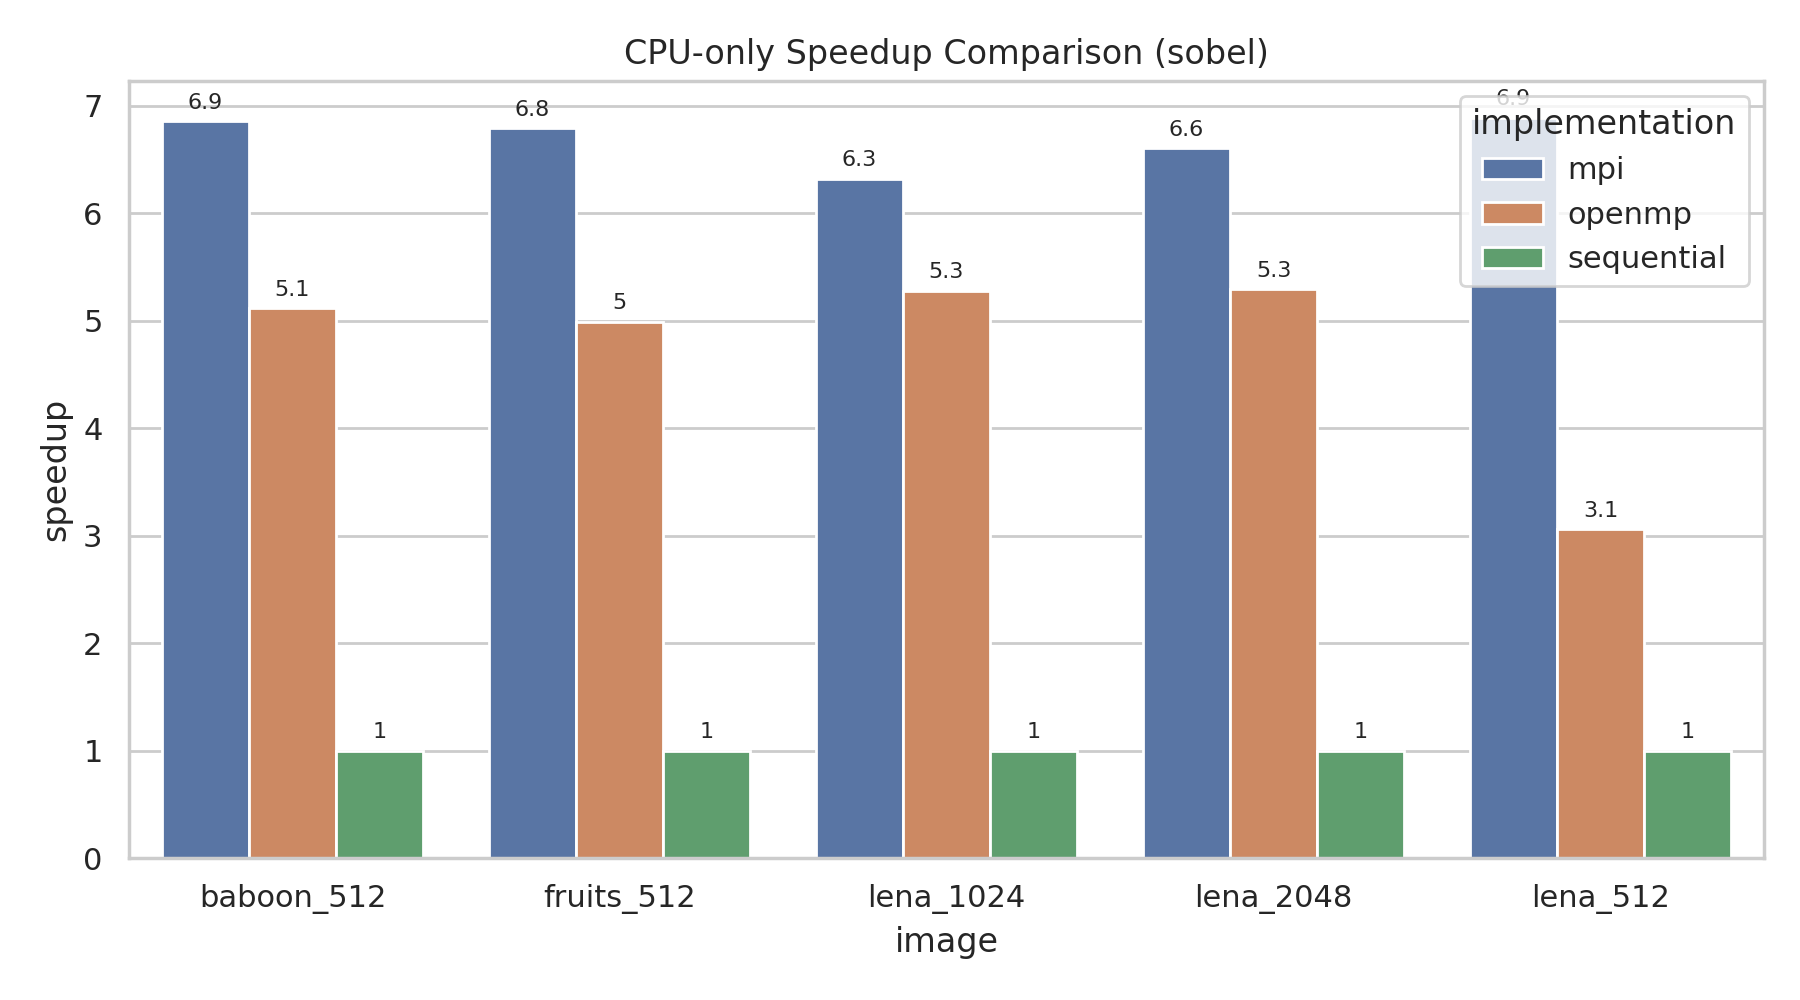
\includegraphics[keepaspectratio,alt={CPU-only speedup (sobel)}]{./plots/output/cpu_only_speedup_sobel.png}}

\pandocbounded{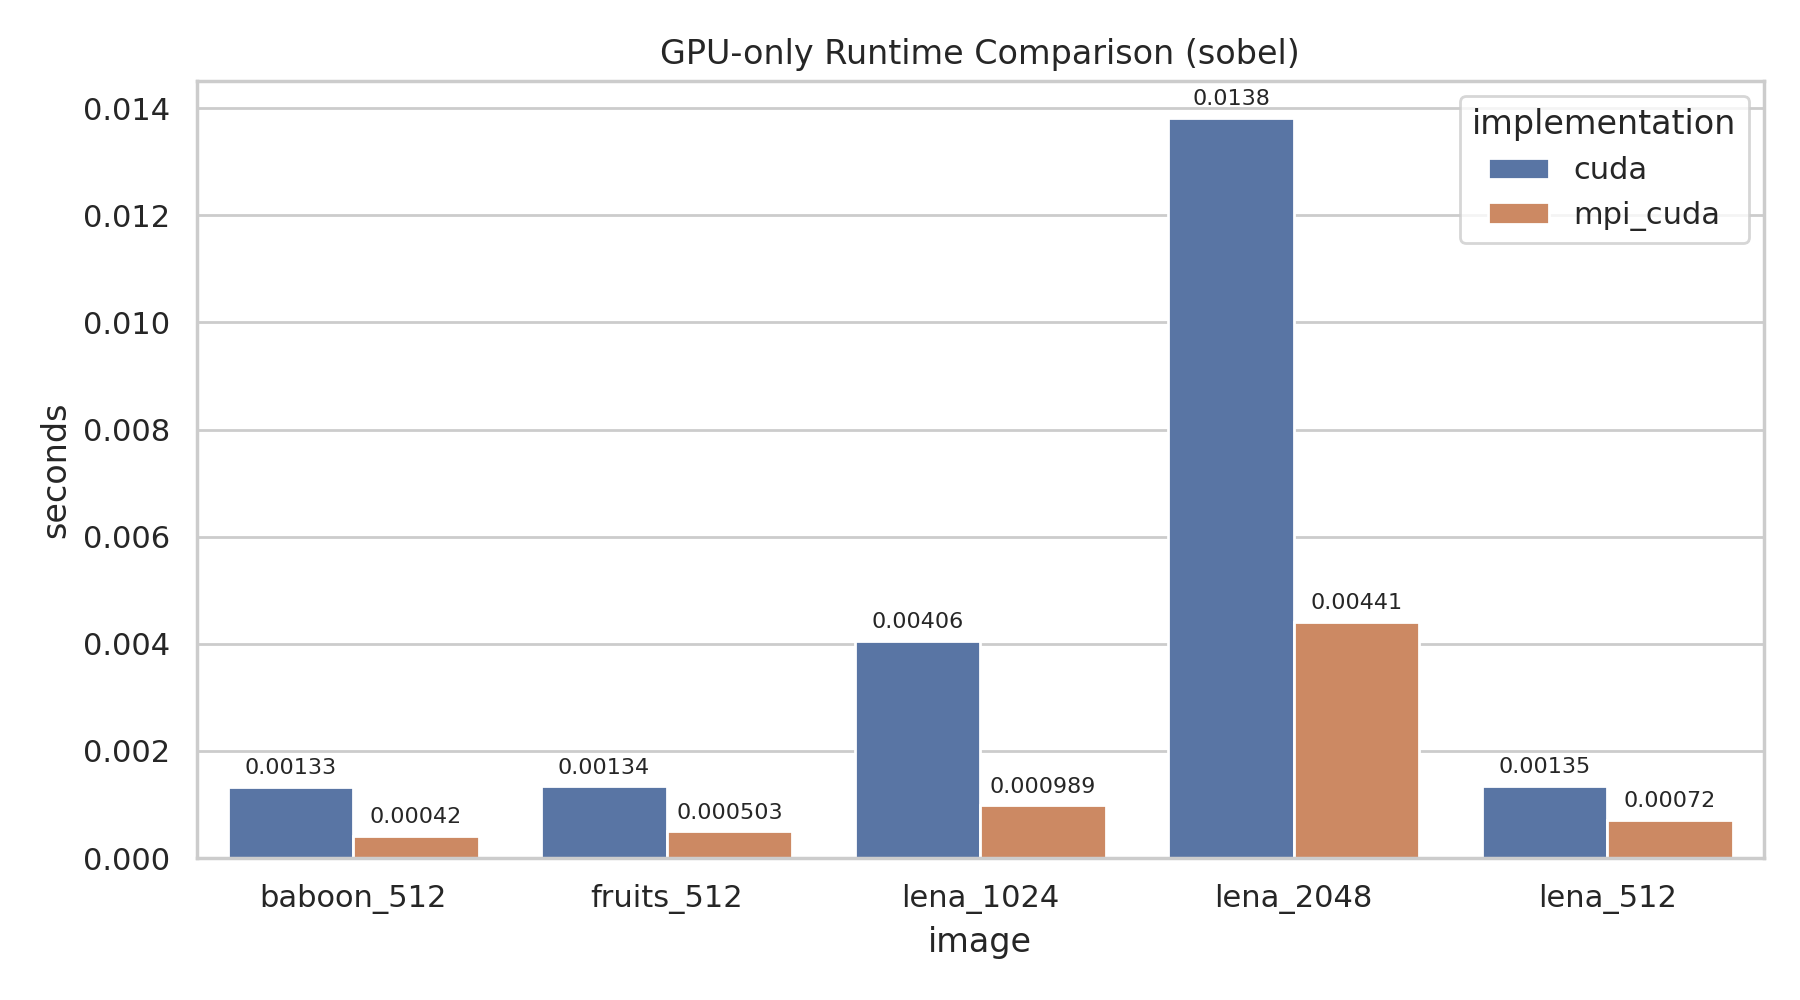
\includegraphics[keepaspectratio,alt={GPU-only runtime (sobel)}]{./plots/output/gpu_only_runtime_sobel.png}}
\pandocbounded{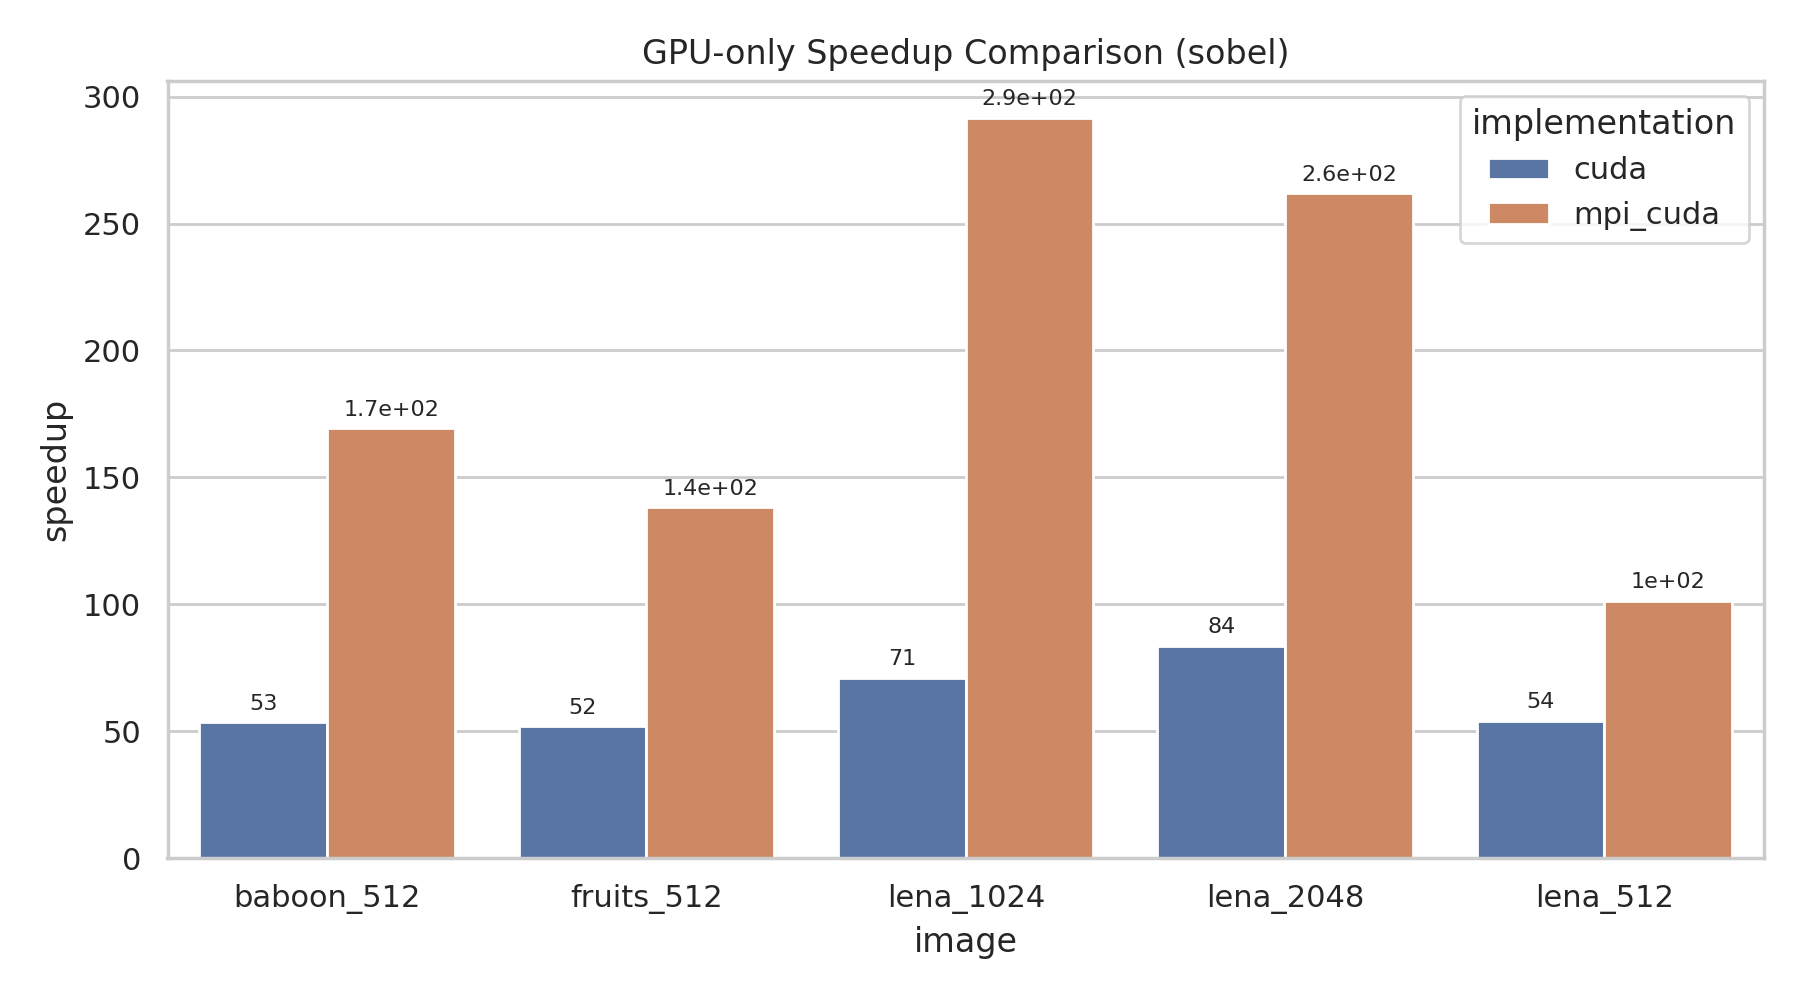
\includegraphics[keepaspectratio,alt={GPU-only speedup (sobel)}]{./plots/output/gpu_only_speedup_sobel.png}}

\pandocbounded{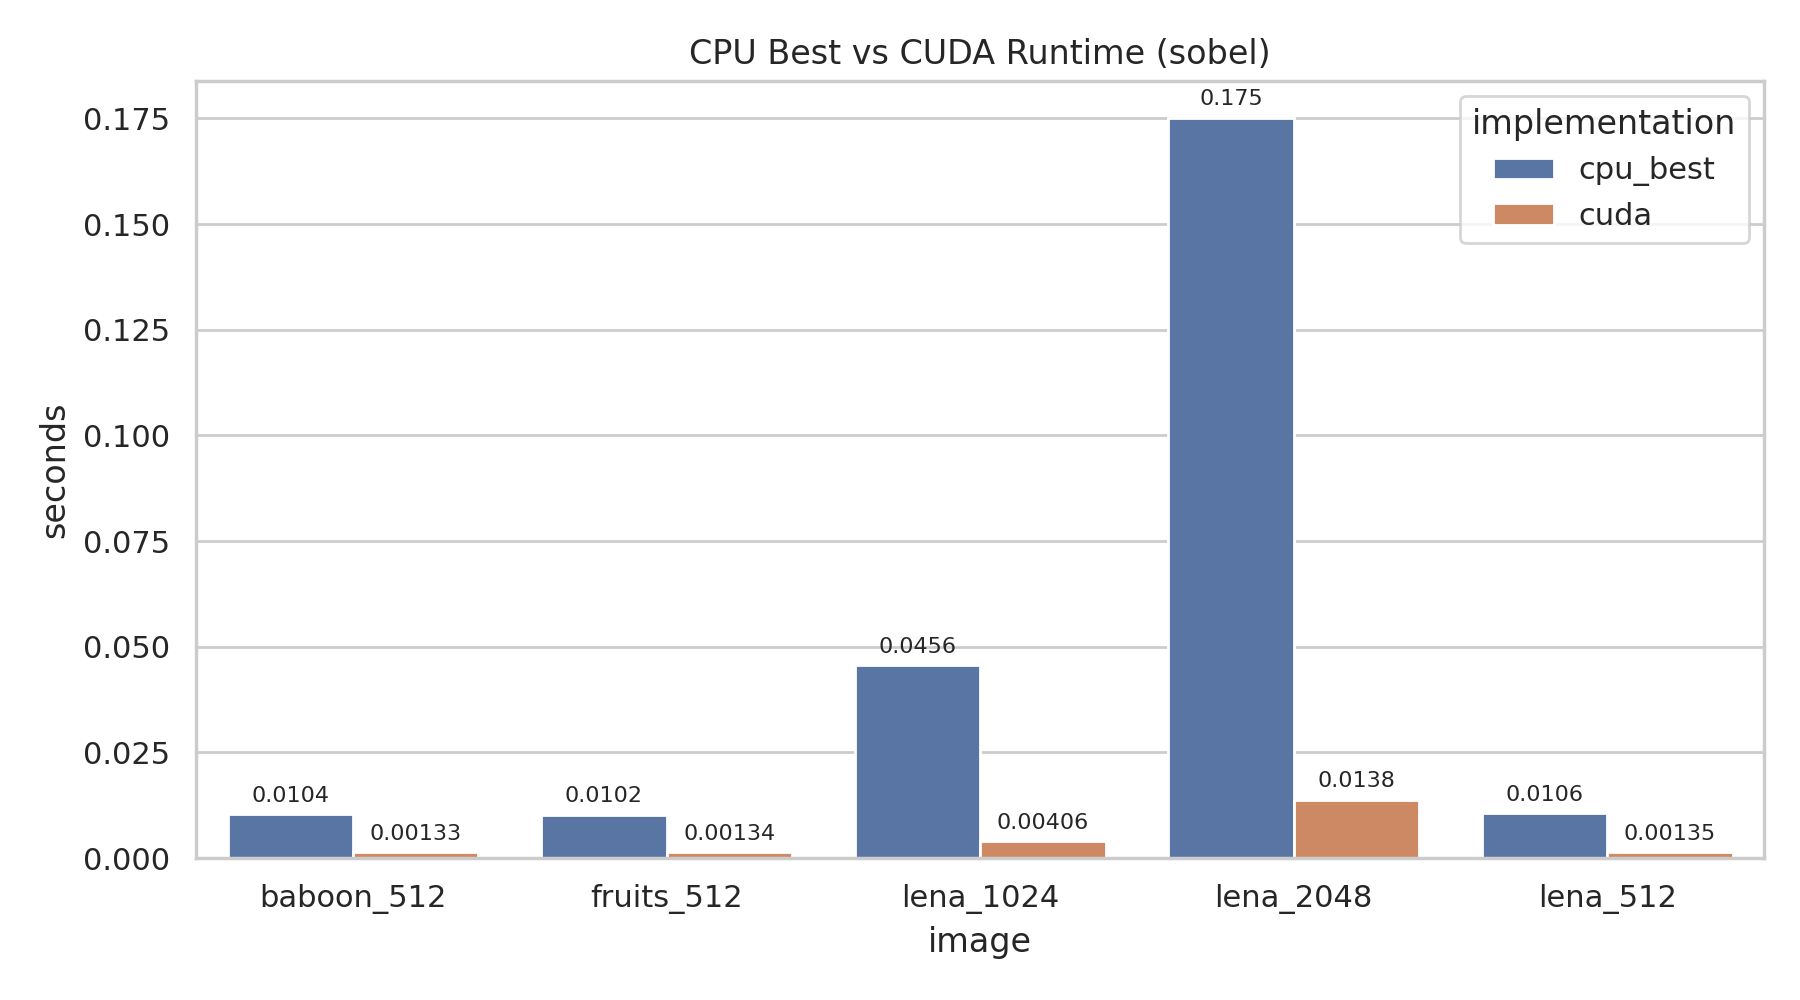
\includegraphics[keepaspectratio,alt={CPU vs CUDA runtime (sobel)}]{./plots/output/cpu_vs_cuda_runtime_sobel.png}}
\pandocbounded{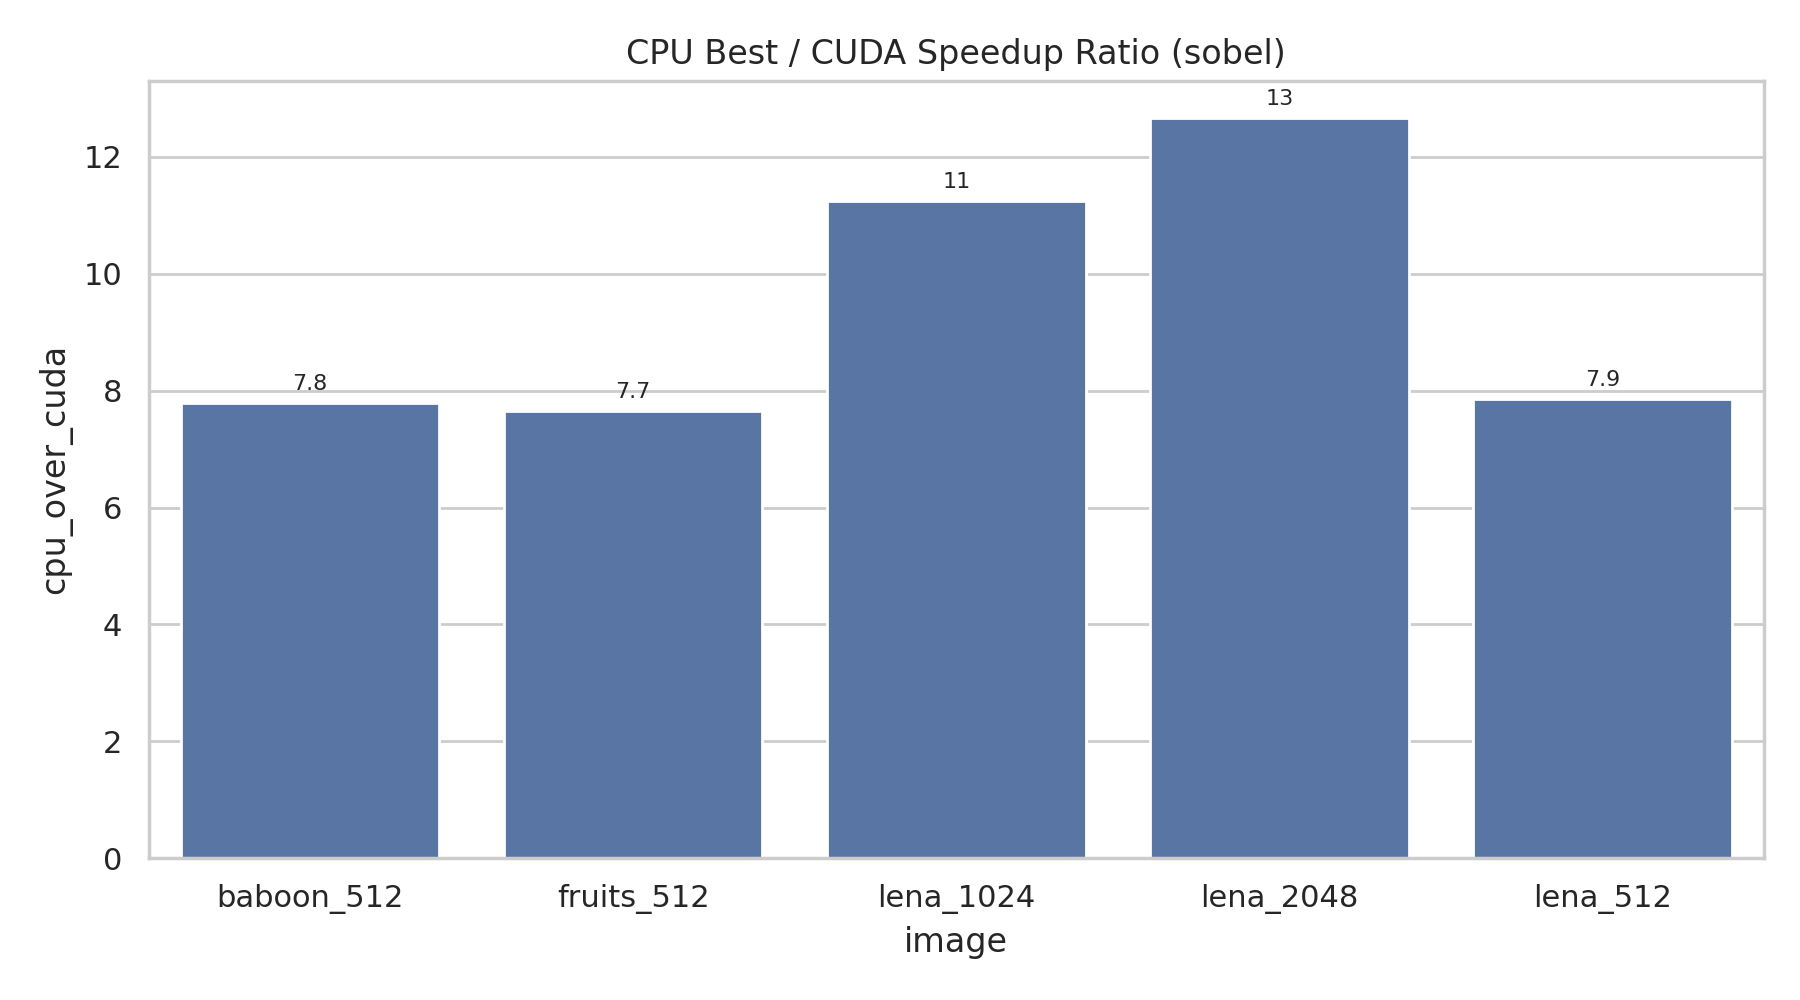
\includegraphics[keepaspectratio,alt={CPU vs CUDA speedup (sobel)}]{./plots/output/cpu_vs_cuda_speedup_sobel.png}}

\pandocbounded{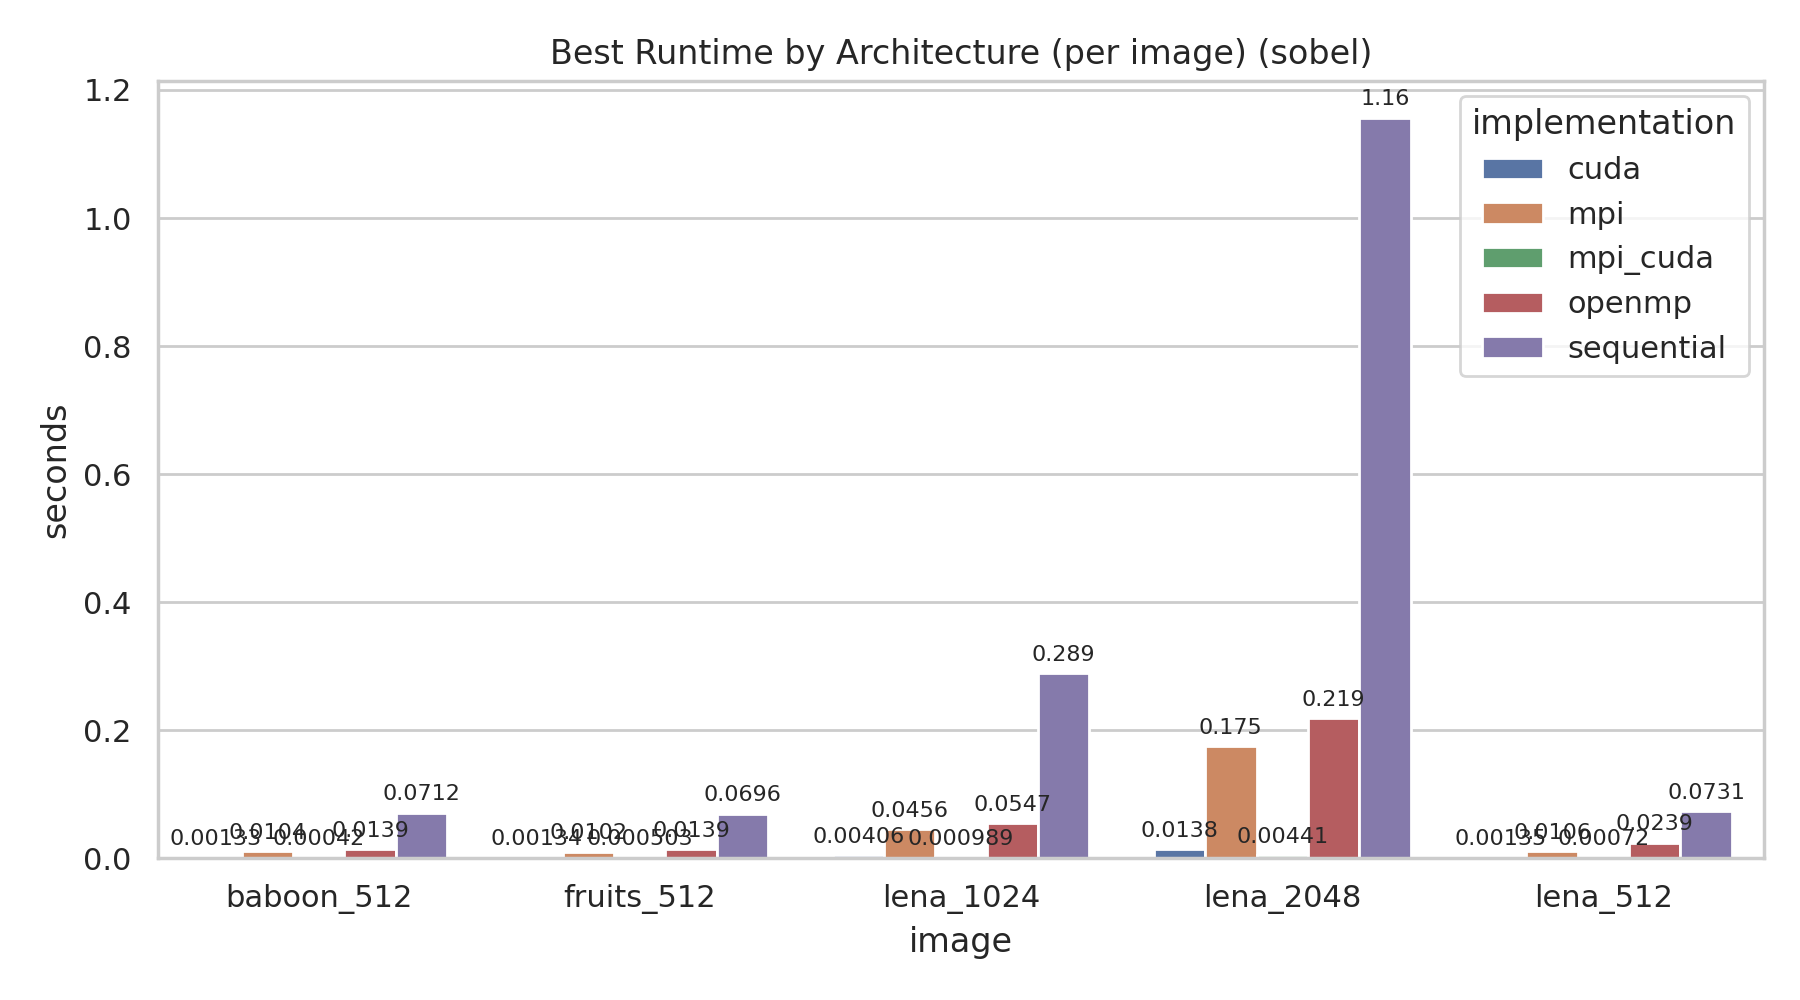
\includegraphics[keepaspectratio,alt={Cross-architecture runtime comparison (sobel)}]{./plots/output/arch_time_comparison_sobel.png}}
\pandocbounded{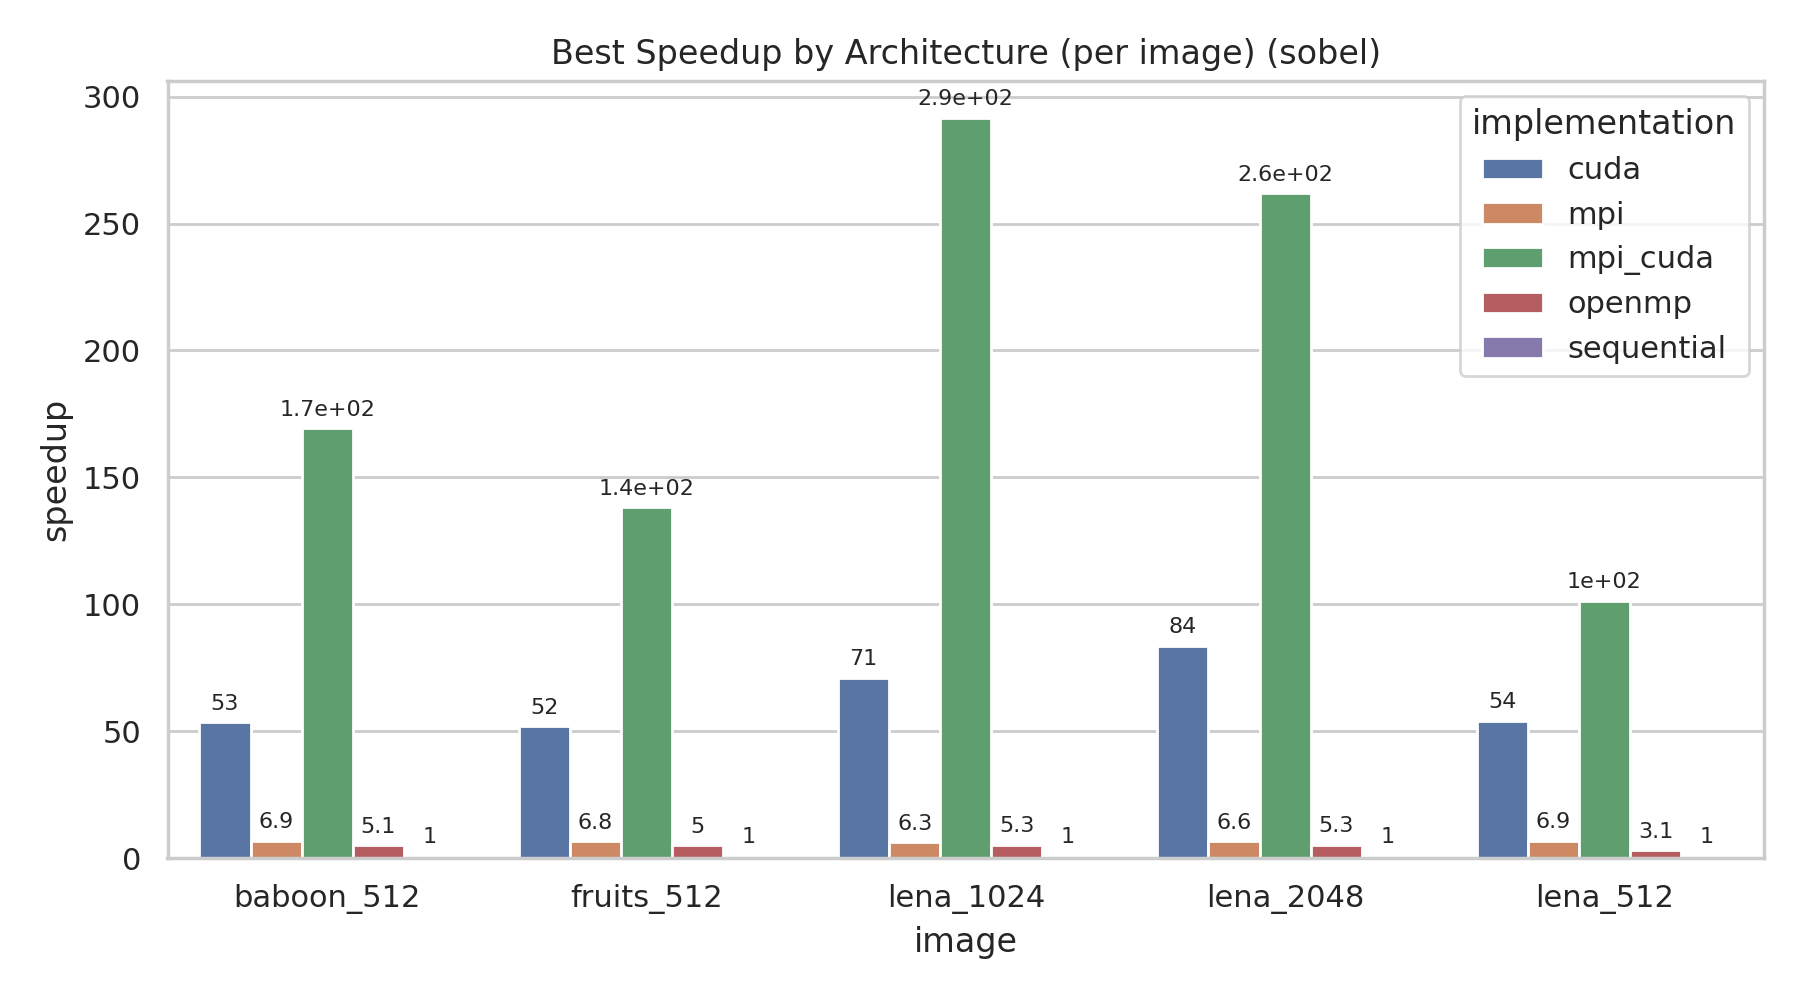
\includegraphics[keepaspectratio,alt={Cross-architecture speedup comparison (sobel)}]{./plots/output/arch_speedup_comparison_sobel.png}}

For interactive exploration, see the notebook
\url{Results_Analysis.ipynb}.

\begin{center}\rule{0.5\linewidth}{0.5pt}\end{center}

\subsection{Conclusion}\label{conclusion}

This case study demonstrates that the same convolution algorithm can
scale from a basic sequential CPU baseline to multi-threaded OpenMP,
distributed MPI, and GPU CUDA implementations. The correctness checks
confirm that all implementations are consistent, while the benchmarks
highlight how different architectures trade off latency, bandwidth, and
overhead.

Most importantly, the step-by-step approach shows how \textbf{parallel
thinking} changes the shape of the solution: not the algorithm itself,
but how we \emph{map} independent work onto different hardware models.

If I were to extend this further, I would add halo-exchange in MPI and
shared-memory tiling in CUDA to reduce global memory traffic even more.

\end{document}
